\documentclass[11pt,french,french]{article}
\usepackage{lmodern}
\usepackage{amssymb,amsmath}
\usepackage{ifxetex,ifluatex}
\usepackage{fixltx2e} % provides \textsubscript
\ifnum 0\ifxetex 1\fi\ifluatex 1\fi=0 % if pdftex
  \usepackage[T1]{fontenc}
  \usepackage[utf8]{inputenc}
\else % if luatex or xelatex
  \ifxetex
    \usepackage{mathspec}
    \usepackage{xltxtra,xunicode}
  \else
    \usepackage{fontspec}
  \fi
  \defaultfontfeatures{Mapping=tex-text,Scale=MatchLowercase}
  \newcommand{\euro}{€}
\fi
% use upquote if available, for straight quotes in verbatim environments
\IfFileExists{upquote.sty}{\usepackage{upquote}}{}
% use microtype if available
\IfFileExists{microtype.sty}{%
\usepackage{microtype}
\UseMicrotypeSet[protrusion]{basicmath} % disable protrusion for tt fonts
}{}
\usepackage[margin=0.95in]{geometry}
\ifxetex
  \usepackage{polyglossia}
  \setmainlanguage{}
\else
  \usepackage[shorthands=off,french]{babel}
\fi
\usepackage{longtable,booktabs}
\ifxetex
  \usepackage[setpagesize=false, % page size defined by xetex
              unicode=false, % unicode breaks when used with xetex
              xetex]{hyperref}
\else
  \usepackage[unicode=true]{hyperref}
\fi
\hypersetup{breaklinks=true,
            bookmarks=true,
            pdfauthor={},
            pdftitle={},
            colorlinks=true,
            citecolor=blue,
            urlcolor=blue,
            linkcolor=magenta,
            pdfborder={0 0 0}}
\urlstyle{same}  % don't use monospace font for urls
\setlength{\parindent}{0pt}
\setlength{\parskip}{6pt plus 2pt minus 1pt}
\setlength{\emergencystretch}{3em}  % prevent overfull lines
\setcounter{secnumdepth}{5}

\providecommand{\tightlist}{%
  %\setlength{\itemsep}{0pt}
  \setlength{\parskip}{0pt}
  }

%%% Use protect on footnotes to avoid problems with footnotes in titles
\let\rmarkdownfootnote\footnote%
\def\footnote{\protect\rmarkdownfootnote}


  \title{Analyse statistique et empirique des modèles\\
de \emph{Word-Embedding} sur Twitter}
    \author{Kim Antunez, Romain Lesauvage, Alain Quartier-la-Tente\\
sous l'encadrement de Benjamin Muller (Inria)}
    \date{}
  
\usepackage{caption}
\usepackage{graphicx}
\usepackage{natbib}
\usepackage[dvipsnames]{xcolor}
\usepackage{fontawesome}
\DeclareMathOperator{\arctanh}{arctanh}
\usepackage{subcaption}
\usepackage{microtype}
\usepackage{amsmath,amssymb}

\begin{document}

\maketitle


{
\hypersetup{linkcolor=black}
\setcounter{tocdepth}{2}
\tableofcontents
}
\newpage 

\section*{Introduction}\label{introduction}
\addcontentsline{toc}{section}{Introduction}

Grâce à l'évolution des méthodes d'apprentissage profond (\emph{Deep
Learning}), l'appréhension du langage naturel est aujourd'hui devenue
une discipline à part entière (\emph{Natural Language Processing}). Ce
succès s'explique en partie grâce à l'émergence de techniques non
supervisées d'apprentissage de représentation de structures
linguistiques. Les méthodes de \emph{word embedding} («~plongement
lexical~» en français) permettent de représenter chaque mot d'un
dictionnaire par un vecteur de nombres réels afin que les mots qui
apparaissent dans des contextes similaires possèdent des vecteurs
correspondants qui sont relativement proches (au sens d'une distance
définie). Les modèles \emph{Word2Vec}, développés par une équipe de
recherche chez Google (\cite{Mikolov}), sont parmi les plus célèbres et
sont ceux sur lesquels se concentrera notre projet.

Dans ce projet de statistique appliquée, nous étudierons dans un premier
temps en détail et implémenterons le modèle \emph{Word2Vec} (partie
\ref{sec:word2vec}). Dans un deuxième temps, nous évaluerons la validité
du modèle implémenté et l'appliquerons sur une base de données composée
de plusieurs millions de tweets publiés en France entre 2013 et 2017
(partie \ref{sec:evaluation}). Enfin, nous mobiliserons des techniques
d'analyse de sentiments afin de créer des indicateurs qui pourront être
comparés aux indicateurs produits dans la statistique publique, en
particulier concernant l'opinion des ménages (partie
\ref{sec:sentimentalAnalysis}).

\section{\texorpdfstring{Implémentation du modèle
\emph{Word2Vec}}{Implémentation du modèle Word2Vec}}\label{sec:word2vec}

\subsection{\texorpdfstring{Le modèle \emph{Word2vec}, un modèle de
\emph{word-embedding}}{Le modèle Word2vec, un modèle de word-embedding}}\label{le-moduxe8le-word2vec-un-moduxe8le-de-word-embedding}

Le \emph{Natural Language Processing} (NLP ou «~traitement automatique
du langage naturel~») est une branche du \emph{machine learning} visant
à analyser, traiter et reproduire le langage humain. Les modèles de NLP
\emph{Word2Vec}, développés par une équipe de recherche chez Google
(\cite{Mikolov}), sont parmi les plus célèbres et utilisent le
\emph{word-embedding} -- plongement lexical en français.

\subsubsection{\texorpdfstring{Historique : de la sémantique vectorielle
à
\emph{Word2Vec}}{Historique : de la sémantique vectorielle à Word2Vec}}\label{historique-de-la-suxe9mantique-vectorielle-uxe0-word2vec}

La «~sémantique vectorielle~» est née dans les années 1950\footnote{L'ouvrage
  \cite{Jurafsky} permet de retracer avec une grande richesse
  l'évolution des méthodes de NLP.}. C'est une méthode algébrique de
représentation d'un document visant à réaliser des tâches diverses
(détecter le plagiat, filtrer des articles\dots). Il est alors
nécessaire de capter de nombreux types de proximités entre mots : les
synonymes (automobile / voiture), antonymes (froid / chaud),
connotations positives \emph{versus} négatives (heureux / triste), etc.

Un modèle répondant à toutes ces exigences ne peut exister. Pour y
répondre au mieux, la sémantique vectorielle puise son inspiration des
travaux linguistiques des années 1950 et en particulier de l'
«~hypothèse de distribution~» selon laquelle un mot se définit par son
environnement. Dit autrement : les mots qui se produisent dans un
contexte identique tendent à avoir des significations
similaires\footnote{Comme l'a écrit le linguiste britannique John Rupert
  Firth en 1957, «~Vous connaîtrez un mot par ses fréquentations~».}.

Les premiers modèles sémantiques (comme le \emph{term frequency-inverse
document frequency} (TF-IDF)) représentaient les relations entre mots
grâce à des très grandes matrices, dites \emph{sparses}, dont les
dimensions correspondaient à la taille du vocabulaire (contenant donc
beaucoup de 0). Les méthodes de \emph{word-embedding} qui sont ensuite
apparues ont permis de représenter chaque mot d'un dictionnaire par un
vecteur de nombres réels denses (peu de 0) de plus faible dimension (en
général entre 50 et 1000). Si la réduction de dimension rend les
vecteurs-mots moins facilement interprétables, elle a pour grand
avantage de faciliter et d'accélérer les tâches d'apprentissage
impliquant ces mots.

\cite{Mikolov} ont mis en avant en 2013 les méthodes de
\emph{word-embedding} à travers la création de \emph{Word2Vec}. Ce
modèle de réseaux de neurones\footnote{C'est l'article \cite{Bengio} qui
  a introduit dix ans avant \emph{Word2Vec} le premier modèle
  d'apprentissage de représentation de vecteurs-mots à partir d'un
  réseau de neurone simple.} à deux couches est rapidement devenu une
référence grâce à la grande précision des résultats qu'il permet
d'obtenir, pouvant être entraîné en un temps record sur un corpus très
volumineux.

\subsubsection{\texorpdfstring{\emph{Word2Vec}, un modèle
d'apprentissage
«~auto-supervisé~»}{Word2Vec, un modèle d'apprentissage «~auto-supervisé~»}}\label{subsec:word2vec}

En sortie du modèle \emph{Word2Vec}, chaque mot est représenté par un
vecteur dont la dimension est fixée par la valeur d'un hyperparamètre.
Les mots qui apparaissent dans des contextes similaires («~bonjour~» et
«~salut~» par exemple) seront représentés par des vecteurs relativement
proches dans l'espace vectoriel de définition de ces vecteurs. Dans la
même logique, \emph{Word2Vec} permet également de réaliser des
opérations vectorielles, comme dans l'exemple, souvent cité :
\(\overrightarrow{Paris} - \overrightarrow{France} + \overrightarrow{Italie} = \overrightarrow{Rome}\)
qui provient de \cite{Mikolov}.

Deux architectures du modèle \emph{Word2Vec} existent (voir graphique
\ref{fig:cbowskipgram}) :

\begin{itemize}
\item
  L'approche \emph{Continuous bags of words} dont l'objectif est
  d'estimer la probabilité d'observer un mot, appelé \textbf{«~focus~»},
  sachant le contexte dans lequel il apparaît (i.e. : les mots
  \textbf{voisins} qualifiés de \textbf{«~contextes~»}).
\item
  L'approche \emph{Skip-gram} a un objectif inverse : estimer, pour
  chaque mot du vocabulaire, la probabilité d'être proche du mot focus.
  C'est cette approche que nous étudions dans ce projet et dans la suite
  de ce rapport. 
\end{itemize}

\begin{figure}[htp]
\centering
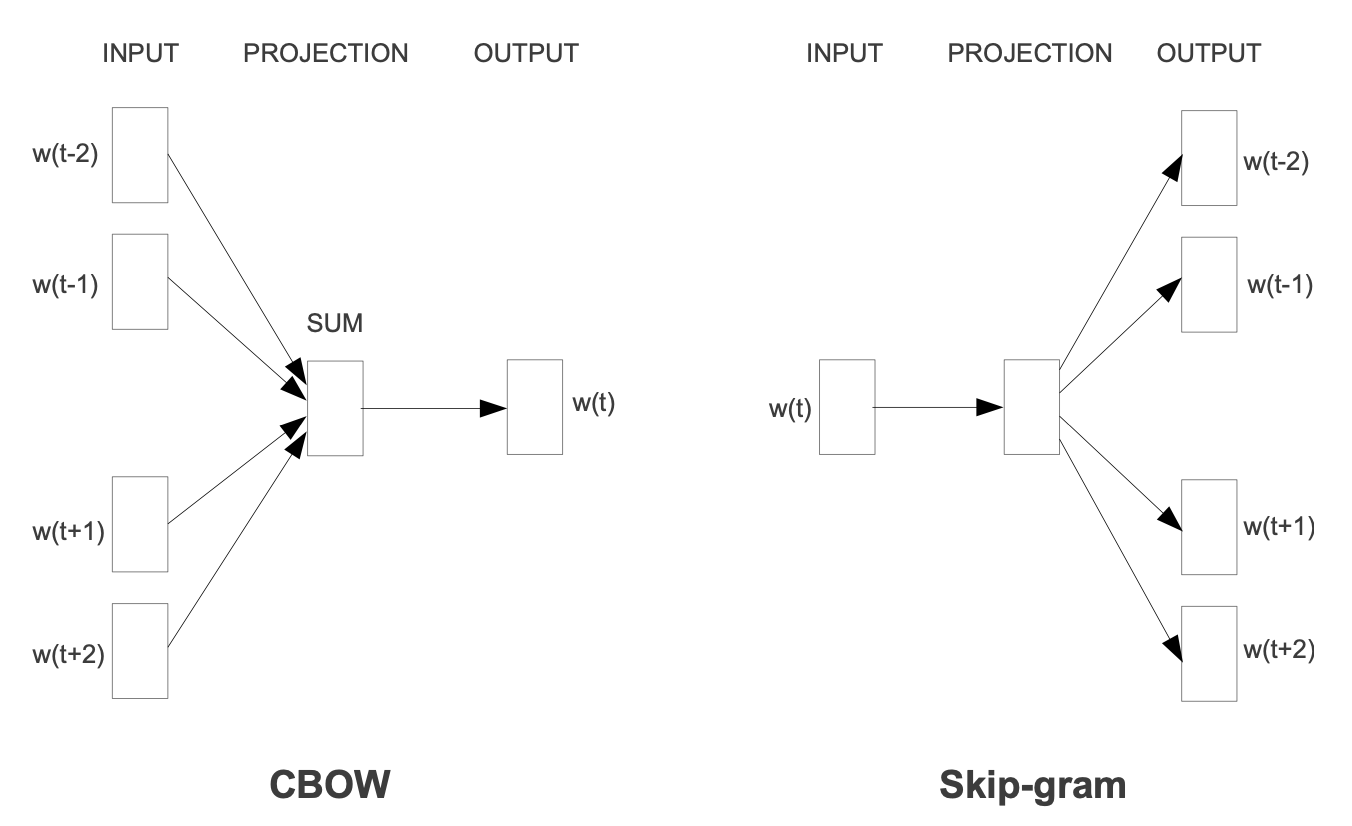
\includegraphics[width=.6\textwidth]{img/cbow_skip_gram.png}
\captionsetup{margin=0cm,format=hang,justification=justified}
\caption{Architecture des modèles Continuous bags of words (CBOW) et Skip-gram.}\label{fig:cbowskipgram}
%\vspace{-0.3cm}
\footnotesize
\emph{Source : \cite{Mikolov}}
\end{figure}

Pour transformer chaque mot en un vecteur, au lieu de simplement compter
les fréquences d'apparition des mots contextes voisins d'un mot
focus\footnote{Comme dans les premiers modèles sémantiques dits
  \emph{sparses}.}, nous entraînons un réseau de neurones sur une tâche
annexe : on construit un classifieur dont la tâche de prédiction est
binaire pour chacun des mots du vocabulaire et répond à la question
(dans le cas Skip-Gram) «~Est-ce que ce mot contexte est susceptible
d'être voisin du mot focus ?~». La prédiction en elle-même ne nous
intéresse pas, c'est plutôt le poids du classifieur en sortie du modèle
qui correspondra aux \emph{word-embeddings}.

Les voisins d'un mot focus reposent sur un hyperparamètre : la fenêtre
(\emph{window} ou \(w\)). Pour \(w = p\), les voisins du mot focus sont
les \(p\) mots précédents et les \(p\) mots suivants dans la phrase. Par
exemple, dans la phrase :

\begin{quote}
\LARGE \textbf{``}\normalsize \emph{Le professeur de statistique est strict avec ses élèves.} \LARGE \textbf{''}\normalsize
\end{quote}

pour \(w=2\), si le mot focus est «~statistique~» alors le contexte qui
lui est associé est : \texttt{{[}professeur,\ de,\ est,\ strict{]}} ; si
le mot focus est «~professeur~» alors le contexte qui lui est associé
est : \texttt{{[}Le,\ de,\ statistique{]}}.

Pour déterminer les représentations vectorielles des mots, nous
entraînons le réseau de neurones en le nourrissant des paires
\texttt{{[}focus,\ contexte{]}}\footnote{Dans notre exemple :
  \texttt{{[}statistique,\ professeur{]},\ {[}statistique,\ de{]}}\dots}
contenues dans les différentes phrases (ici tweets) du corpus afin qu'il
puisse déterminer les probabilités d'apparition d'un mot dans le
voisinage d'un autre mot (voir description de l'algorithme en partie
\ref{sec:skipgram}).

Ainsi, la grande force du modèle d'apprentissage \emph{Word2Vec} est
qu'il est «~auto-supervisé~». En effet, comme nous avons vu plus haut,
le corpus est considéré comme une donnée d'entraînement implicitement
supervisée, ce qui nous évite d'avoir à mobiliser des corpus annexes
annotés.

\subsection{L'algorithme Skip-Gram}\label{sec:skipgram}

L'objectif de cette partie est de décrire le fonctionnement de
l'approche Skip-gram.

Dans la suite de ce projet nous noterons \(n\) la taille du vocabulaire
(i.e. : le nombre de mots différents) et \(dim\) la dimension retenue
pour les \emph{word-embeddings}. Comme décrit dans la partie
\ref{subsec:word2vec}, l'approche \emph{Skip-gram} peut être vue comme
un réseau de neurones à deux couches avec :

\begin{itemize}
\item
  En entrée une matrice \(W_e\) de taille \(n\times dim\) ;
\item
  En sortie une matrice \(W_S\) de taille \(n\times dim\).
\end{itemize}

Ces deux matrices sont initialisées en générant des lois normale
\(\mathcal N(0,1)\). Elles sont ensuite mises à jour, grâce aux couples
\texttt{{[}focus,\ contexte{]}} construits à partir du contexte (voir
partie \ref{subsec:baseentrainement}), par un algorithme de descente de
gradient. À la fin de l'algorithme, ce sont ces matrices qui donneront
la représentation vectorielle des mots du vocabulaire. Ainsi, la ligne
\(i\) de la matrice \(W=\frac{W_e+W_s}{2}\) donnera la représentation du
\(i\)\textsuperscript{ème} mot du vocabulaire en dimension \(dim\).

\subsubsection{Construction de la base
d'entraînement}\label{subsec:baseentrainement}

Peu de traitements sont effectués sur la base initiale : nous mettons
tout en minuscule, remplaçons les ponctuations par des espaces, mais
laissons tous les chiffres et les accents. Chaque phrase\footnote{Dans
  notre cas une phrase correspond à un tweet, même si ce tweet peut être
  composé de plusieurs phrases.} est ensuite \emph{tokénisée} par la
chaîne de caractère correspondant à un espace \texttt{"\ "} : on
considère qu'il y a autant de mots de que chaînes de caractères séparées
par un espace\footnote{Les mots composés sont donc considérés comme
  plusieurs mots distincts.}. Par exemple, la phrase :

\begin{quote}
\LARGE \textbf{``}\normalsize \emph{Que pensez-vous de CE projet?(i.e. : qu'avez-vous retenu en 10min ?)} \LARGE \textbf{''}\normalsize
\end{quote}

est décomposée en 14 mots
\texttt{{[}que,\ pensez,\ vous,\ de,\ ce,\ projet,\ i,\ e,\ qu,\ avez,\ vous,\ retenu,\ en,\ 10min{]}}.

Comme décrit dans la partie \ref{subsec:word2vec}, les couples
\texttt{{[}focus,\ contexte{]}} dépendent d'un hyperparamètre : la
fenêtre \(w\). Pour éviter que les mots trop fréquents, souvent peu
informatifs (comme les pronoms personnels), soient sur-entraînés, deux
traitements sont effectués :

\begin{enumerate}
\def\labelenumi{\arabic{enumi}.}
\item
  Pour chaque phrase on effectue un sous-échantillonnage
  (\emph{subsampling}). Pour chaque mot \(w_i\) on note \(z(w_i)\) la
  proportion d'apparition de ce mot, c'est-à-dire le rapport entre le
  nombre de fois que ce mot apparaît et le nombre total de mots. La
  probabilité de garder un mot le mot \(w_i\) est donnée par : \[
  \mathbb P(w_i) = \min\left\{\left(\sqrt{\frac{z(w_i)}{q}} + 1 \right)
  \times
  \frac{q}{z(w_i)},1\right\}
  \] Le paramètre \(q\) appelé «~sample~» -- échantillonnage -- contrôle
  le nombre de mots sous-échantillonnés (plus il est grand, plus la
  probabilité de garder le mot \(w_i\) est grande). Si \(q\) vaut 0,001
  (valeur par défaut) alors par exemples :

  \begin{itemize}
  \tightlist
  \item
    \(\mathbb P(w_i) = 1\) (\(w_i\) est toujours gardé) lorsque
    \(z(w_i)\leq 0,0026\), c'est-à-dire si \(w_i\) représentent moins de
    0,26 \% du nombre total de mots.\\
  \item
    \(\mathbb P(w_i) = 0,5\) (50 \% de chance de garder \(w_i\)) lorsque
    \(z(w_i)=0,00746\).\\
  \item
    \(\mathbb P(w_i) = 0,033\) (3,3 \% chance de garder \(w_i\)) lorsque
    \(z(w_i)=1,0\) (si le corpus n'est constitué que du mot \(w_i\), ce
    qui serait bien sûr absurde).
  \end{itemize}
\end{enumerate}

Ce sous-échantillonnage est effectué de manière indépendante pour chaque
phrase : un même mot peut donc être sous-échantillonné dans une phrase
et ne pas l'être dans une autre.

\begin{enumerate}
\def\labelenumi{\arabic{enumi}.}
\setcounter{enumi}{1}
\tightlist
\item
  Pour chaque phrase, on tire au hasard (selon une loi uniforme) un mot
  focus pour lequel on tire un mot \emph{contexte} au hasard dans la
  fenêtre \(w\), en imposant que les deux mots choisis soient parmi les
  mots sous-échantillonnés\footnote{Si pour une phrase, aucun couple
    \texttt{{[}focus,\ contexte{]}} ne figurent simultanément dans les
    mots sous-échantillonnés, alors aucun couple n'est retenu pour cette
    phrase.}. Par exemple, nous supposons que dans la phrase
  \texttt{{[}que,\ pensez,\ vous,\ de,\ ce,\ projet,\ i,\ e,\ qu,\ avez,\ vous,\ retenu,\ en,\ 10min{]}},
  les mots sous-échantillonnés sont les mots en position 2, 5, 6, 8, 9,
  10, 11, 12, 13, 14. Pour mieux comprendre, nous remplaçons les mots
  non échantillonnés par «~nonsubsampled~». La phrase devient alors
  \texttt{{[}nonsubsampled,\ pensez,\ nonsubsampled,\ nonsubsampled,\ ce,\ projet,\ nonsubsampled,\ e,\ qu,\ avez,\ vous,\ retenu,\ en,\ 10min{]}}.
  Si \(w=2\) alors le mot focus tiré ne peut pas être «~pensez~» puisque
  dans ce cas il n'y aurait aucun mot contexte associé. Si le mot focus
  tiré est «~qu~» alors le mot contexte est tiré au hasard parmi
  \texttt{{[}e,\ avez,\ vous{]}}.
\end{enumerate}

Ce mécanisme va être répété sur toutes les phrases du corpus et
l'ensemble du corpus va être parcouru plusieurs fois. Le nombre de fois
que l'ensemble du corpus est parcouru est appelé \emph{epochs}.

\subsubsection{Descente de gradient}\label{subsec:descentedegradient}

Pour chaque couple \texttt{{[}focus,\ contexte{]}}, les matrice \(W_e\)
et \(W_s\) sont mises à jour par descente de gradient. C'est-à-dire que
\(\theta^{(t)} = W_e\) et \(\theta^{(t)} = W_s\), les matrices obtenues
après la \(t\)\textsuperscript{ème} itération de l'algorithme, sont
mises à jour par l'équation :
\[\theta^{(t+1)} = \theta^{(t)} - \eta \nabla_\theta Loss(\theta^{(t)})\]
avec \(\eta\) le taux d'apprentissage (un hyperparamètre à fixer) et
\(L(\theta)\) la fonction de perte.

Le modèle \emph{Word2vec} a initialement été construit en utilisant une
fonction de perte dérivée de la fonction \emph{softmax} (voir partie
\ref{subsec:softmax} et \cite{Mikolov}). L'algorithme a ensuite été
amélioré en utilisant le \emph{negative sampling} (voir partie
\ref{subsec:negsampling} et \cite{MikolovNS}).

\paragraph{Version softmax}\label{subsec:softmax}

Soit \(w_1,\,\dots,\,w_T\) les mots utilisés pour entraîner le modèle.
L'objectif du modèle Skip-Gram est, étant donné un mot focus, de prévoir
quels sont les mots voisins contextes dans une certaine fenêtre \(w\).
Mathématiquement, on cherche à maximiser la quantité :

\begin{equation*}
\frac 1 T\sum_{t=1}^T\sum_{-w\leq j \leq w,\,j\ne 0} \log \mathbb P(w_{t+j}\vert w_{t})
\label{eq:objSoftMax}
\end{equation*}

où :

\begin{itemize}
\item
  les \(w_{t+j}\) sont les mots voisins de \(w_t\) (\(w_t\) est donc un
  mot focus et \(w_{t+j}\) un mot contexte) ;
\item
  \(\mathbb P(w_{t+j}\vert w_{t})\) est la probabilité d'observer le mot
  contexte \(w_{t+j}\) sachant que l'on a observé le mot focus \(w_t\).
  Cette quantité est calculée en fonction des matrices \(W_e\) et
  \(W_s\) à partir de la fonction softmax \footnote{Étant donné le
    vecteur \(z=(z_1,\,\dots,\,z_n)\)) la fonction softmax est la
    fonction qui à \(z\) associe le vecteur dont la
    \(j\)\textsuperscript{ème} coordonnée est égale à
    \(\frac{\exp(z_j)}{\sum_{i=1}^n\exp(z_i)}\).}. En notant \(n\) la
  taille du vocabulaire et \(W_{e,w_i}\) et \(W_{s,w_i}\) les
  représentations vectorielles du mot \(w_i\) respectivement dans la
  matrice d'entrée et de sortie, cette probabilité est égale à\footnote{Dans
    tout le rapport nous utiliserons la notation \(^{t}X\) pour désigner
    la transposée de la matrice \(X\).} : \[
  \mathbb P(w_{contexte}\vert w_{focus}) = 
  \frac{
  \exp(W_{e,w_{focus}}\times {}^tW_{s,w_{contexte}})
  }{
  \sum_{i=1}^n\exp(W_{e,w_{focus}}\times {}^tW_{s,w_{i}})
  }
  \]
\end{itemize}

Maximiser l'équation \eqref{eq:objSoftMax} revient à minimiser la fonction
de perte suivante pour chaque couple {[}focus, contexte{]} :

\[
Loss_{1}=-\log\mathbb P(w_{contexte}\vert w_{focus}) =
-W_{e,w_{focus}}\times {}^tW_{s,w_{contexte}}+
\log\left(\sum_{i=1}^n\exp(W_{e,w_{focus}}\times {}^t W_{s,w_i})\right)
\] L'inconvénient de cette méthode est qu'elle est très gourmande en
temps de calcul. En effet, pour chaque couple
\texttt{{[}focus,\ contexte{]}}, la complexité du calcul de
\(\log\mathbb P(w_{contexte}\vert w_{focus})\) est proportionnelle à la
taille du vocabulaire. La taille du vocabulaire pouvant être très grande
(par exemple, dans notre base de tweets, cette taille est de 70 330), le
temps de calcul peut vite devenir très important.

C'est pourquoi la version \emph{softmax} est très peu utilisée dans les
implémentations de Skip-Gram. Une approche alternative, \emph{negative
sampling} avec une fonction sigmoïde, moins gourmande en temps de
calcul, est alors souvent préférée\footnote{Une autre alternative à
  l'approche \emph{softmax} parfois utilisée est l'approche
  \emph{hierarchical softmax} qui se base sur l'utilisation d'arbres
  binaires de classification. La complexité de cet algorithme est
  proportionnelle à \(\log_2n\) mais reste plus importante que celle de
  l'approche \emph{negative sampling}.}.

\paragraph{\texorpdfstring{Version \emph{negative
sampling}}{Version negative sampling}}\label{subsec:negsampling}

Le \emph{negative sampling} est basé sur le concept du \emph{Noise
Contrastive Estimation} -- estimation contrastée du bruit -- où on
cherche, à partir d'un modèle logistique, à différencier un vrai signal
(un vrai couple \texttt{{[}focus,\ contexte{]}}) d'un faux (un bruit qui
correspondrait à un faux couple \texttt{{[}focus,\ contexte{]}} généré
aléatoirement).

Dans cette approche, plutôt que de mettre à jour l'ensemble des
représentations vectorielles des mots pour chaque couple
\texttt{{[}focus,\ contexte{]}}, on tire \(K\) mots au hasard du
vocabulaire \((w_{neg,\,i})_{i=1..K}\), selon une loi \(P\) (définie
plus tard), en considérant que ces mots ne seront pas des mots voisins
de \texttt{focus}\footnote{Il est bien sûr possible que parmi les mots
  tirés au hasard il y ait des mots qui soient vraiment dans le
  contexte. Cependant, puisque la taille du vocabulaire est très grande,
  on considère que cette erreur est négligeable.}.

L'approche \emph{softmax} peut être vue comme un problème de
classification multiclasses : étant donné un mot \texttt{focus}, on
estime la probabilité que les autres mots soient parmi ses voisins
(chaque classe étant un mot du vocabulaire). L'idée du \emph{negative
sampling} est de transformer ce problème de classification multiclasses
en un problème de classification binaire d'une variable \(D\) : pour
chaque couple \texttt{{[}focus,\ mot2{]}}, on cherche à déterminer si
\texttt{mot2} est dans le contexte de \texttt{focus}. Si c'est le cas,
alors \(D=1\) (mot2 est positif et est le \texttt{contexte}), sinon
\(D=0\) (mot2 est négatif, il appartient à \((w_{neg,\,i})_{i=1..K}\)).

On cherche donc à maximiser
\(\mathbb P(D=1\vert w_{focus},w_{contexte})\) et
\(\mathbb P(D=0\vert w_{focus},w_{neg,\,i})\). Pour estimer ces
probabilités, on utilise une fonction sigmoïde plutôt que la fonction
softmax : \[
\mathbb P(D=1\vert w_{focus},w_{contexte})=\sigma(W_{e,w_{focus}}{}^tW_{s,w_{contexte}}) = 
\frac{1}{1+\exp(-W_{e,w_{focus}}{}^tW_{s,w_{contexte}})}
\] et : \[
\mathbb P(D=0\vert w_{focus},w_{neg,\,i})=\sigma(-W_{e,w_{focus}}{}^tW_{s,w_{neg,\,i}}) = 
\frac{1}{1+\exp(W_{e,w_{focus}}{}^tW_{s,w_{neg,\,i}})}
\] Par rapport à l'approche \emph{softmax}, on cherche toujours à
maximiser la quantité de l'équation \eqref{eq:objSoftMax} mais en estimant
\(\log\mathbb P(w_{contexte}\vert w_{focus})\) par : \[
\log\mathbb P(w_{contexte}\vert w_{focus}) =
\log\underbrace{\sigma (W_{e,w_{focus}}{}^tW_{s,w_{contexte}})}_{
\mathbb P(D=1\vert w_{focus},w_{contexte})
}+
\sum_{i=1}^K\mathbb E_{w_{neg,i}\sim P}[
\log
\underbrace{\sigma (-W_{e,w_{focus}}{}^tW_{s,w_{neg,\,i}})}_{
\mathbb P(D=0\vert w_{focus},w_{neg,\,i})
}
]
\]

Ainsi, pour chaque couple \texttt{{[}focus,\ contexte{]}} et un ensemble
\((w_{neg,\,i})_{i=1..K}\) de mots négatifs tirés, on associe la
fonction de perte suivante, à minimiser : \[
Loss_{2}=-\log\sigma (W_{e,w_{focus}}{}^tW_{s,w_{contexte}})
-
\sum_{i=1}^K
\log
\sigma (-W_{e,w_{focus}}{}^tW_{s,w_{neg,\,i}})
\] La complexité est ici bien plus faible que pour la fonction softmax
puiqu'elle est proportionnelle à \(K\).

\cite{MikolovNS} trouvent, empiriquement, que la meilleure distribution
\(P\) pour générer les mots négatifs est telle que : \[
\mathbb P_P(w_i) = \frac{z(w_i)^{3/4}}{
\sum_{j=1}^n z(w_j)^{3/4}
}
\]

Avec \(z(w_i)\) la fréquence d'apparition du mot \(w_i\).

Ils recommandent également de prendre \(K\in\{5,\dots,20\}\) pour les
petites bases de données et \(K\in\{2,\dots,5\}\) pour les grandes bases
de données. Dans ce projet, nous utiliserons \(K=5\) (pour chaque couple
\texttt{{[}focus,\ contexte{]}} nous tirons donc 5 mots négatifs).

\section{Évaluation du modèle implémenté}\label{sec:evaluation}

Malgré l'utilisation généralisée des \emph{word embeddings}, très peu de
travaux théoriques expliquent ce qui est réellement capturé par ces
représentations de mots.

C'est pourquoi ce modèle est principalement évalué à l'aide de méthodes
empiriques. Les méthodes que nous avons retenues pour évaluer, dans les
parties qui suivent, la qualité des vecteurs-mots obtenus sont décrites
plus précisément dans l'annexe \ref{annexe:commentEvaluer}.

\subsection{Évaluation sur un corpus fictif}\label{sec:corpusFictif}

Avant de nous attaquer au jeu de données complet décrit plus bas, nous
avons évalué un premier corpus fictif afin de nous assurer de la
robustesse et de la validité du modèle implémenté. Nous avons associé
dix couples (du type {[}voiture, camion{]}), à dix mots contextes
différents ({[}véhicule, moto\dots{]}). Le corpus fictif est formé de 10
000 phrases composées chacune d'un mot d'un couple, de cinq mots du
contexte et de trois mots bruits, tous tirés aléatoirement.

Nous avons ensuite mis en œuvre les différentes techniques
d'évaluation\footnote{À l'exception de la méthode par \og jugement
  humain \fg{} puisque le corpus est ici créé fictivement par ordinateur
  sans prêter attention au réel sens des mots.} présentées en partie
\ref{sec:commentEvaluer} sur les \emph{word-embeddings} obtenus grâce à
ce corpus fictif.

\begin{table}
\begin{center}
\begin{tabular}{|c|c|c|}
    \hline
    mot & similarité cosinus \tabularnewline
    \hline
    énorme & 0,991   \tabularnewline
    taille & 0,991   \tabularnewline
    \dots & \dots    \tabularnewline
    vanille & 0,061   \tabularnewline
    salissures & 0,054   \tabularnewline
    \hline
 \end{tabular}
\captionsetup{margin=0cm,format=hang,justification=justified}
\caption{Mots les plus proches de \og grand \fg{} par similarité cosinus}\label{table:tableau_evaluation}
\end{center}
\vspace{-0.3cm}
\footnotesize
\emph{Note : Paramètres utilisés : ep = 50 / lr = 0,01 / w = 5 / dim = 10.}
\end{table}

Les résultats semblent concluants : la similarité cosinus montre bien
une forte corrélation entre les mots focus et contexte du corpus initial
et une faible corrélation avec les mots bruits (tableau
\ref{table:tableau_evaluation}). L'ACP et l'algorithme t-SNE permettent
également de montrer graphiquement cette proximité
(figure~\ref{fig:figure_evaluation}). Les clusters apparaissent de
manière plus évidente avec t-SNE.

\begin{figure}
\begin{center}
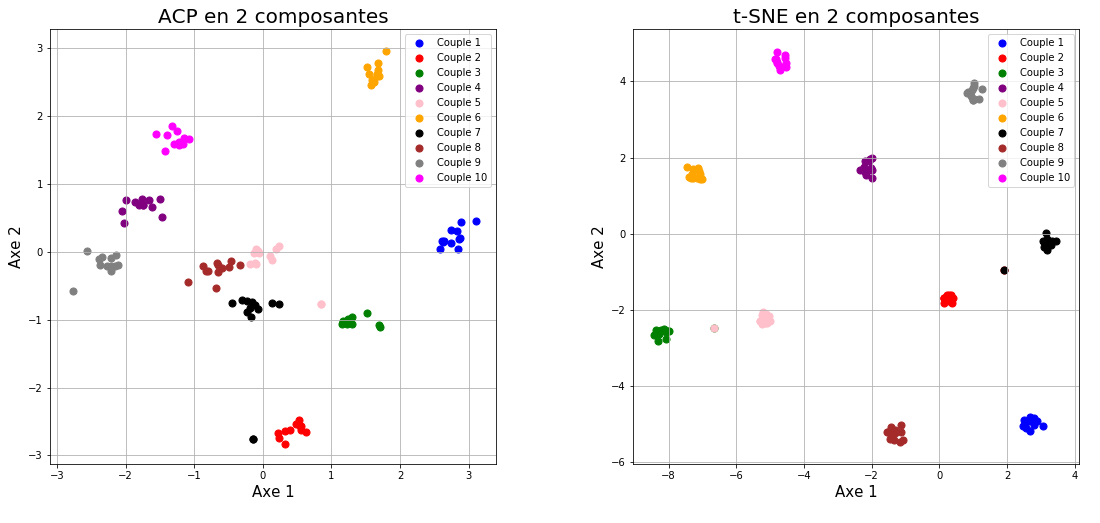
\includegraphics[width=1\textwidth]{img/figures.png}
\captionsetup{margin=0cm,format=hang,justification=justified}
\caption{Évaluation du modèle sur données fictives}\label{fig:figure_evaluation}
\end{center}
\vspace{-0.3cm}
\footnotesize
\emph{Note : Paramètres utilisés : ep = 50 / lr = 0,01 / w = 5 / dim = 10.}
\end{figure}

\subsection{Choix des meilleurs hyperparamètres pour le
modèle}\label{choix-des-meilleurs-hyperparamuxe8tres-pour-le-moduxe8le}

Une fois nous être assurés de la bonne implémentation du modèle (partie
\ref{sec:corpusFictif}) grâce au corpus fictif, nous nous sommes
attachés à identifier les hyperparamètres les plus pertinents au regard
des données dont nous disposons.

Ces données correspondent à un ensemble de 1,3 million de
tweets\footnote{Ces tweets, achetés à twitter, sont la propriété de
  l'Inria.} postés en France entre 2014 et 2017, supposés être
représentatifs de l'ensemble de tweets nationaux publiés durant cette
période.

Le modèle \emph{Word2Vec} version Skip-gram, décrit en partie
\ref{sec:word2vec}, fait en effet intervenir un certain nombre
d'hyperparamètres parmi lesquels :

\begin{itemize}
\item $ep$ : le nombre d'\og \emph{epochs} \fg{}
\item $lr$ ou $\alpha$ : le \og \emph{learning rate} \fg{}, ou taux d'apprentissage
\item $w$ (\emph{window}): la taille de la fenêtre de sélection des mots contextes
\item $dim$ : la dimension des vecteurs-mots (ou \emph{word-embeddings})
\end{itemize}

Or, la performance de nombreuses méthodes de \emph{machine learning},
dont \emph{Word2Vec}, dépend fortement des valeurs choisies pour ces
paramètres, ces valeurs étant elles-mêmes très dépendantes des données
mobilisées.

Même si les méthodes d'optimisation bayésiennes deviennent de plus en
plus performantes pour optimiser la valeur de ces hyperparamètres en
tenant compte de leurs interactions (\cite{Hutter}), ce choix s'effectue
régulièrement de manière empirique, en testant différentes valeurs
d'hyperparamètres sur les données mobilisées. C'est l'approche que nous
retenons ici.

Le package \texttt{Gensim} (\og Generate Similar \fg{}), dans lequel la
méthode \emph{Word2Vec} est implémentée, est un des outils actuels les
plus robustes et performants\footnote{Grâce à sa dépendance à
  \texttt{NumPy}, \texttt{Gensim} puise dans des bibliothèques de bas
  niveau. Ainsi, alors que le code de haut niveau est du Python, c'est
  en fait du Fortran et du C hautement optimisés qui sont utilisés, ce
  qui rend \texttt{Gensim} bien plus performant que \texttt{PyTorch} que
  nous avons utilisé pour implémenter le modèle décrit en partie
  \ref{sec:word2vec}.} pour la modélisation sémantique non supervisée
(\cite{Rehurek}).

Nous avons choisi de mobiliser \texttt{Gensim} dans la suite de ce
rapport, en parallèle du modèle que nous avons implémenté, en raison de
son temps d'exécution bien plus rapide\footnote{À titre d'exemple, alors
  qu'une epoch sur l'ensemble des tweets met une vingtaine d'heures à
  tourner pour \og notre \fg{} modèle, elle met 1 minute via
  \texttt{Gensim}.}. Cette rapidité d'exécution nous a permis de
réaliser des tests d'hyperparamètres plus nombreux.

Pour réaliser ces tests, nous avons fait tourner le modèle
\emph{Word2Vec} plusieurs fois en modifiant un à un les paramètres. Nous
avons ensuite évalué ces différents modèles par la méthode du
\og jugement humain \fg{} (voir partie \ref{sec:jugementHumain}) en
comparant la mesure de la similarité cosinus\footnote{Nous avons
  également évalué les modèles en utilisant (l'inverse de) la distance
  euclidienne à la place de la similarité cosinus. L'effet des
  paramètres devient alors bien moins clair et la performance du modèle
  est inférieure, ce va dans le sens de l'utilisation plus fréquente de
  la méthode de la similarité cosinus dans la littérature.} entre deux
mots obtenue à partir de notre modèle à l'évaluation subjective de cette
proximité par des individus. En outre, un même modèle est lancé six fois
(six \og seeds \fg{} différentes) afin de construire des intervalles de
confiance de la matière décrite précédemment, en empilant les six
échantillons de mesure de proximités correspondant aux six
implémentations d'un même modèle\footnote{Pour chaque modèle, nous
  calculons les statistiques de rang des 65 paires de mots de la base de
  jugement humain ainsi que le rang des similarités cosinus des mots
  obtenus en sortie du modèle. Nous réalisons ces actions pour les six
  implémentations du même modèle et empilons les résultats obtenus.
  C'est à partir de cette base empilée de 6x65 lignes moins les données
  manquantes que nous calculons chaque intervalle de confiance selon la
  formule décrite en partie \ref{sec:jugementHumain}.}.

\subsubsection{Nombre d'epochs, taille de fenêtre et taux
d'apprentissage}\label{nombre-depochs-taille-de-fenuxeatre-et-taux-dapprentissage}

Pour cette première série de tests d'hyperparamètres, nous avons fixé la
dimension des \emph{word-embeddings} à 50\footnote{En réalisant les
  mêmes tests sur uniquement 100 000 tweets, puis en testant une
  dimension de \emph{word-embeddings} de 20, les effets observés et
  commentés ici se confirment.} et évalué l'impact du nombre d'epochs,
de la taille de la fenêtre et du taux d'apprentissage (figure
\ref{fig:evaluation_1}) .

\begin{figure}
\begin{center}
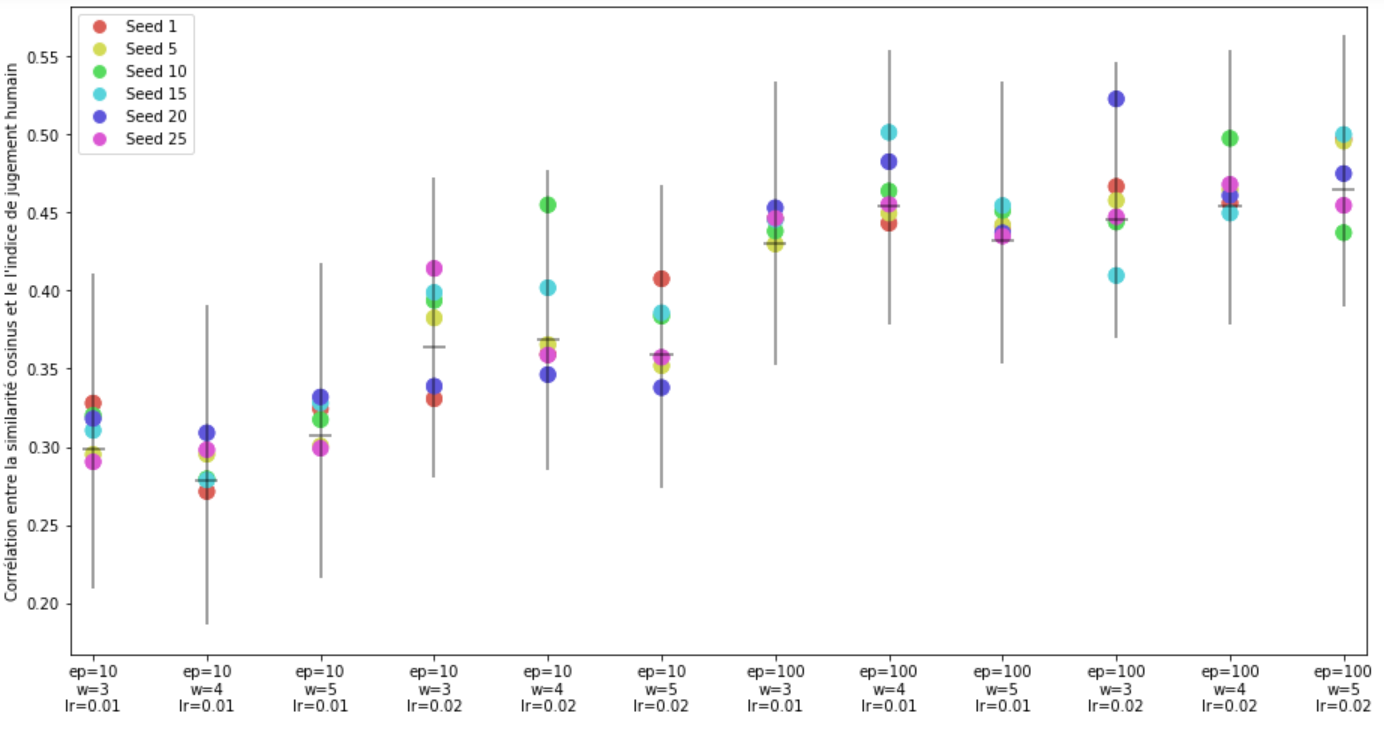
\includegraphics[width=1\textwidth]{img/test_parametres.png}
\captionsetup{margin=0cm,format=hang,justification=justified}
\caption{Tests d'hyperparamètres : epochs, fenêtre et taux d'apprentissage}\label{fig:evaluation_1}
\end{center}
\vspace{-0.3cm}
\footnotesize
\emph{Note : Paramètres utilisés : dim = 50\newline
Le trait horizontal correspond au coefficient de Spearman calculé sur les échantillons empilés des six modèles et la barre verticale à l'intervalle de confiance associé.}
\end{figure}

\paragraph{Le nombre d'epochs}\label{le-nombre-depochs}

~

Le nombre d'epochs a un effet net. Passer de 10 à 100 epochs fait
nettement augmenter le score de corrélation de Spearman entre données
subjectives et données en sortie du modèle.

\faArrowCircleRight{} Nous retenons alors le paramètre \textbf{ep =
100}.

\paragraph{Le taux d'apprentissage}\label{le-taux-dapprentissage}

~

La valeur 0,02 semble donner systématiquement de meilleurs résultats que
0,01. En réalisant davantage de tests de taux d'apprentissage en fixant
les autres hyperparamètres, les différents taux d'apprentissage
présentent des performances similaires\footnote{En fixant les paramètres
  dim = 50, ep = 100 et w = 4 (celles du modèle retenu \emph{in fine}),
  et en testant les taux d'apprentissage 0,005, 0,01, 0,02, 0,03 et
  0,04, les valeurs moyennes des corrélations s'échelonnent entre 0,41
  et 0,48, soit des valeurs proches.}.

\faArrowCircleRight{} Nous retenons alors le paramètre \textbf{lr =
0,02}.

\paragraph{La taille de la fenêtre}\label{la-taille-de-la-fenuxeatre}

~

La taille de la fenêtre ne semble pas jouer un rôle majeur, et dépend
beaucoup des autres paramètres choisis.

Certains travaux (\cite{Levy2}) indiquent que, suivant la taille de
fenêtre choisie, les informations capturées sont différentes. Cela
pourrait expliquer la complexité de choisir la \og meilleure \fg{}
taille de fenêtre. Alors que les \og grandes \fg{} fenêtres capturent
des informations sur le domaine du mot (autres mots de tout type étant
utilisés dans des discussions connexes), les \og petites \fg{} fenêtres
saisissent davantage le mot en lui-même (ses extensions, synonymes, lui
sont alors proches). La valeur de 4 représente une taille de fenêtre
\og ni trop grande ni trop petite\fg{} et qui présente de bons résultats
dans la plupart des tests effectués.

\faArrowCircleRight{} Nous retenons alors le paramètre \textbf{w = 4}.

\subsubsection{Dimension des
vecteurs-mots}\label{dimension-des-vecteurs-mots}

On cherche cette fois-ci à évaluer l'effet de la dimension des
\emph{word-embeddings}. Selon certains papiers (comme
\cite{Pennington}), la qualité des représentations vectorielles
s'améliore à mesure que l'on augmente la taille du vecteur, mais
seulement jusqu'à atteindre 300 dimensions\footnote{La dimension des
  vecteurs doit également être adaptée à la taille du vocabulaire. Un
  des articles fondateurs de word2vec (\cite{Mikolov}) recommande donc
  d'augmenter à la fois la dimension des vecteurs et la quantité de
  données d'apprentissage. Par exemple, avec un vocabulaire d'une
  centaine de mots, il serait inefficace d'utiliser des projections en
  grande dimension (risque de surapprentissage).}. Après 300 dimensions,
la qualité des vecteurs commence à diminuer et le temps de calcul
augmente considérablement.

\begin{figure}
\begin{center}
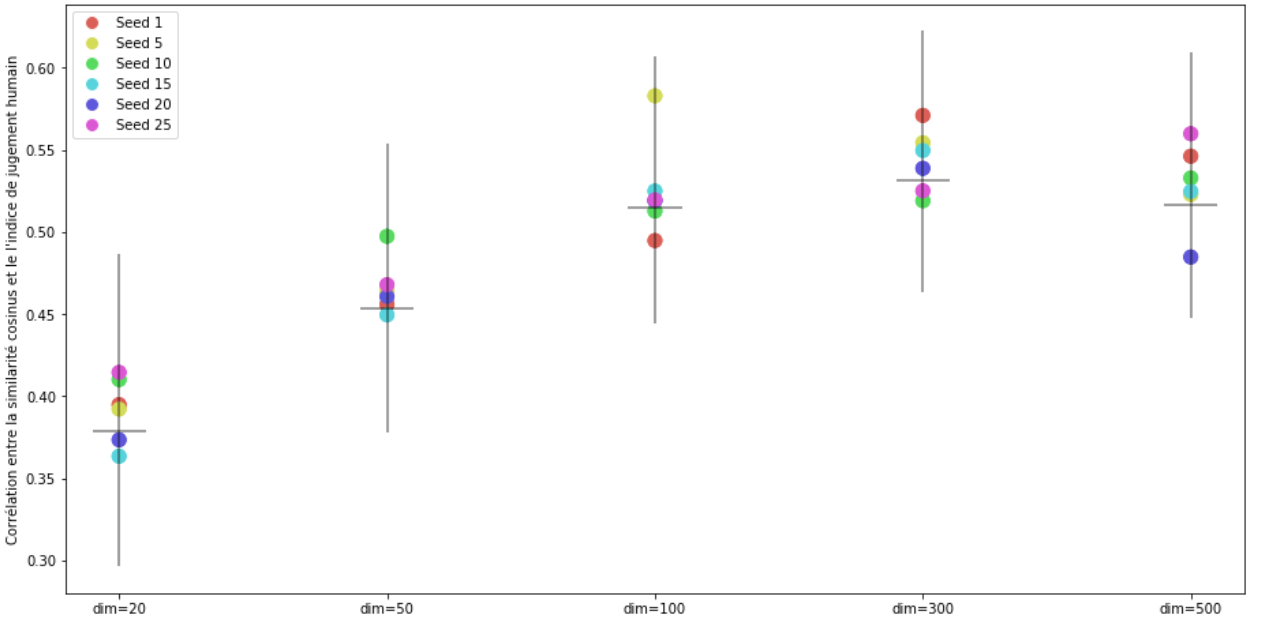
\includegraphics[width=1\textwidth]{img/test_parametres2.png}
\captionsetup{margin=0cm,format=hang,justification=justified}
\caption{Tests d'hyperparamètres : dimension des *word-embeddings*}\label{fig:figure_dim}
\end{center}
\vspace{-0.3cm}
\footnotesize
\emph{Note : Paramètres utilisés : ep = 100 / w = 4 / lr = 0,02.\newline
Le trait horizontal correspond au coefficient de Spearman calculé sur les échantillons empilés des six modèles et la barre verticale à l'intervalle de confiance associé.}
\end{figure}

En pratique, en comparant l'effet de la dimension des vecteurs (modèle
fixé à ep~=~100, w~=~4 et lr~=~0,02), on observe bien une augmentation
de l'efficacité du modèle jusqu'en dimension 300 et une efficacité
moindre en dimension 500 (figure~\ref{fig:figure_dim}). Bien que
l'efficacité du modèle semble meilleure en dimension 300, la dimension
100 améliore la rapidité de l'algorithme, pour des résultats d'une
qualité similaire.

\faArrowCircleRight{} Nous retenons alors le paramètre \textbf{dim =
100}.

\subsection{Évaluation sur le corpus
final}\label{uxe9valuation-sur-le-corpus-final}

\subsubsection{\texorpdfstring{Avec \og notre \fg{}
modèle}{Avec notre  modèle}}\label{avec-notre-moduxe8le}

Nous avons ensuite fait tourner le modèle que nous avons implémenté en
utilisant les paramètres retenus précédemment\footnote{w~=~4, lr~=~0,02
  et dim~=~100} mais uniquement sur 100~000 tweets et 80 epochs pour des
questions de temps de calcul\footnote{Près de 18 heures.}.

Les résultats obtenus semblent relativement satisfaisants. La recherche
des plus proches voisins par similarité cosinus (dont quelques exemples
sont illustrés en tableau \ref{table:knn_ark}) donne des résultats
proches de l'intuition.

\begin{table}
\begin{center}
\begin{tabular}{|c|c|c|c|}
    \hline
\textbf{bonjour} & \textbf{femme} & \textbf{1} & \textbf{samedi} \tabularnewline
\emph{(669 apparitions)} & \emph{(264 apparitions)} & \emph{(765 apparitions)} & \emph{(203 apparitions)} \tabularnewline
       \hline

\includegraphics[height=4mm]{img/emojis/1.png} (0,59) & quelle (0,49) & 5 (0,55) & soir (0,57) \tabularnewline

\includegraphics[height=4mm]{img/emojis/2.png} (0,59) & cette (0,46) & mois (0,51) & vivement (0,51) \tabularnewline
merci (0,54) & une (0,44) & 10 (0,49) & demain (0,50) \tabularnewline
nuit (0,48) & vie (0,44) & 2 (0,48) & end (0,48) \tabularnewline
bisous (0,47) & grippe (0,44) & top (0,48) & weekend (0,47) \tabularnewline
bonne (0,47) & belle (0,43) & depuis (0,47) & matin (0,45) \tabularnewline

\includegraphics[height=4mm]{img/emojis/3.png} (0,46) & ma (0,43) & saison (0,46) & jeudi (0,45) \tabularnewline
vous (0,46) & magnifique (0,43) & ans (0,44) & prochain (0,43) \tabularnewline
plaisir (0,44) & nouvelle (0,43) & jours (0,43) & week (0,43) \tabularnewline
allez (0,43) & vidéo (0,39) & 3 (0,43) & 
\includegraphics[height=4mm]{img/emojis/4.png} (0,42) \tabularnewline
    \hline
 \end{tabular}
\captionsetup{margin=0cm,format=hang,justification=justified}
\caption{10 plus proches voisins par similarité cosinus avec \og notre \fg{} modèle}\label{table:knn_ark}
\end{center}
\vspace{-0.3cm}
\footnotesize
\emph{Note : Paramètres utilisés : ep = 80 / w = 4 / lr = 0,02 / dim = 100 / base : 100 000 tweets\newline
La similarité cosinus de chaque paire de mots est renseignée entre les parenthèses.}

\end{table}

Par ailleurs, le coefficient de Spearman entre la similarité cosinus des
mots obtenus et le jugement humain est de 0,571 (p-valeur : 4,1 \%).
Toutefois, ce bon résultat est à considérer avec précaution puisque
seuls 13 des couples de mots de la base RG-65 ont été reconnus dans le
corpus de 100~000 tweets que nous utilisons ici.

Enfin, les représentations graphiques des positions des mots via des ACP
et les sommes vectorielles sur les mots\footnote{Comme l'exemple de
  \(\overrightarrow{Paris} - \overrightarrow{France} + \overrightarrow{Italie} = \overrightarrow{Rome}\)
  dans \cite{Mikolov}} donnent des résultats bien moins concluants que
le modèle \texttt{Gensim} entraîné sur l'ensemble des tweets (voir
partie \ref{sec:gensimresultats}).

\subsubsection{\texorpdfstring{Avec le modèle
\texttt{Gensim}}{Avec le modèle Gensim}}\label{sec:gensimresultats}

Le modèle \texttt{Gensim}\footnote{w~=~4, lr~=~0,02, dim~=~100 et
  ep~=~100.} donne des résultats encore plus convaincants que
précédemment, ayant été davantage entraîné, et sur un corpus plus fourni
(ensemble des tweets). En effet, les vecteurs-mots en sortie du modèle
\texttt{Gensim} sur l'ensemble des tweets (figure
\ref{fig:acp_freq_gensim}) sont davantage répartis dans l'ensemble du
plan, alors que les mots en sortie du modèle que nous avons implémenté
sur 100 000 tweets sont répartis en fonction de leur nombre
d'occurrences, les mots les moins fréquents n'ayant probablement pas (ou
peu) été entraînés (figure \ref{fig:acp_freq_ark}).

\begin{figure}
\begin{minipage}{.5\textwidth}
  \centering
  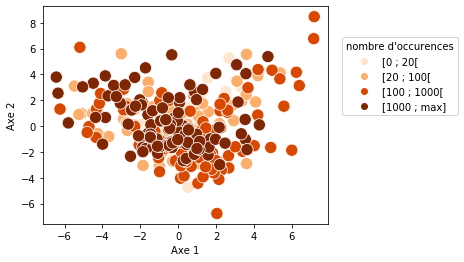
\includegraphics[width=1\linewidth]{img/acp_freq_gensim.png}
  \captionof{figure}{Position des mots en fonction de\newline leur nombre d'occurrences (Modèle \texttt{Gensim})}
  \label{fig:acp_freq_gensim}
\end{minipage}%
\begin{minipage}{.5\textwidth}
  \centering
  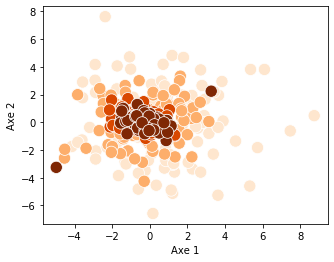
\includegraphics[width=0.72\linewidth]{img/acp_freq_ark.png}
  \captionof{figure}{Position des mots en fonction de\newline leur nombre d'occurrences (\og notre \fg{} modèle)}
  \label{fig:acp_freq_ark}
\end{minipage}
\footnotesize
\emph{Note : Paramètres utilisés : ep = 100 (gauche) ou 80 (droite) / w = 4 / lr = 0,02 / dim = 100.\newline
Méthode utilisée : ACP, deux premiers axes.}
\end{figure}

Le coefficient de Spearman a une valeur semblable à précédemment : 0,495
mais sa p-valeur est proche de 0 \% et, cette fois-ci, 52 des couples de
mots de la base RG-65 ont été reconnus dans le corpus de tweets.

Les 10 plus proches voisins calculés par similarité cosinus (tableau
\ref{table:knn_gensim}) semblent encore davantage pertinents. Les plus
proches voisins de \og \(1\) \fg{} contiennent davantage de chiffres, de
\og samedi \fg{} davantage de jours de la semaine et le tableau contient
désormais des synonymes de \og femme \fg{} et de \og bonjour \fg{}.
Certains mots surprenants subsistent toutefois, comme par exemple
\og transmets \fg{}, \og désagrément \fg{} et \og betembourg \fg{},
voisins de \og bonjour \fg{}. Toutefois, la fréquence d'apparition de
ces mots dans le corpus est faible (moins d'une centaine d'occurrences).
La projection de certains vecteurs-mots sur les deux premiers axes d'une
ACP (figure \ref{fig:acp_gensim}) nous confirme la qualité de
l'entraînement du corpus sur l'ensemble de tweets.

\begin{table}
\begin{center}
\begin{tabular}{|c|c|c|c|}
    \hline
\textbf{bonjour} & \textbf{femme} & \textbf{1} & \textbf{samedi} \tabularnewline
\emph{(17 043 apparitions)} & \emph{(6 177 apparitions)} & \emph{(21 055 apparitions)} & \emph{(4 917 apparitions)} \tabularnewline
       \hline
bonsoir (0,85) & fille (0,86) & 2 (0,65) & vendredi (0,88) \tabularnewline
bjr (0,75) & copine (0,74) & 3 (0,64) & jeudi (0,86) \tabularnewline
hello (0,71) & meuf (0,71) & 6 (0,63) & lundi (0,83) \tabularnewline
salut (0,66) & demoiselle (0,66) & 4 (0,62) & mercredi (0,83) \tabularnewline
coucou (0,55) & nana (0,66) & 7 (0,60) & dimanche (0,83) \tabularnewline
transmets (0,49) & nièce (0,66) & 5 (0,58) & mardi (0,76) \tabularnewline
désagrément (0,48) & sœur (0,65) & 9 (0,58) & demain (0,72) \tabularnewline
avezvous (0,48) & barbe (0,65) & 8 (0,56) & barathon (0,56) \tabularnewline
bettembourg (0,48) & maman (0,64) & 1e (0,55) & 22h45 (0,55) \tabularnewline
hey (0,47) & princesse (0,64) & 34 (0,53) & 20h (0,54) \tabularnewline
    \hline
 \end{tabular}
\captionsetup{margin=0cm,format=hang,justification=justified}
\caption{10 plus proches voisins par similarité cosinus avec le modèle \texttt{Gensim}}\label{table:knn_gensim}
\end{center}
\vspace{-0.3cm}
\footnotesize
\emph{Note : Paramètres utilisés : ep = 100 / w = 4 / lr = 0,02 / dim = 100 / base : ensemble des tweets\newline
La similarité cosinus de chaque paire de mots est renseignée entre les parenthèses.}
\end{table}

\begin{figure}
\begin{center}
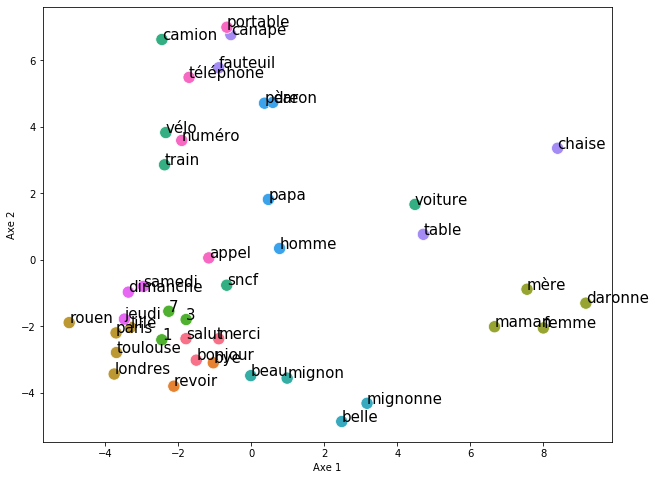
\includegraphics[width=0.5\textwidth]{img/acp_gensim.png}
\captionsetup{margin=0cm,format=hang,justification=justified}
\caption{ACP sur un corpus réduit de mots}\label{fig:acp_gensim}
\end{center}
\vspace{-0.3cm}
\footnotesize
\emph{Note : Paramètres utilisés : ep = 100 / w = 4 / lr = 0,02 / dim = 100 / base : ensemble des tweets }
\end{figure}

Enfin, nous avons réalisé des opérations sur les mots-vecteurs. Si
l'opération
\(\overrightarrow{Roi} - \overrightarrow{Homme} + \overrightarrow{Femme} = \overrightarrow{Reine}\)
(figure \ref{fig:acp_reine}) semble fonctionner \footnote{Les
  similarités cosinus obtenues sont les suivantes :
  \(corr(\overrightarrow{Roi}, \overrightarrow{Homme}) = 0,34\),
  \(corr(\overrightarrow{Homme}, \overrightarrow{Femme}) = 0,35\) et
  \(corr(\overrightarrow{Roi} - \overrightarrow{Homme} + \overrightarrow{Femme} , \overrightarrow{Reine}) = 0,67\).
  \(\overrightarrow{Reine}\) est bien le mot le plus proche de la somme
  vectorielle calculée.}, l'opération
\(\overrightarrow{Paris} - \overrightarrow{France} + \overrightarrow{Italie}\)
(figure \ref{fig:acp_rome}) n'identifie pas \og Rome \fg{}(similarité
cosinus de 0,18 seulement) dans les mots les plus proches mais d'autres
villes comme \og Lyon \fg{} (similarité cosinus de 0,62). \og Rome \fg{}
semble effectivement située \og trop en haut\fg{} dans le plan de l'ACP
par rapport aux autres villes. Peut-être ce mot n'a-t-il pas
suffisamment été entraîné (246 apparitions dans les tweets contre 46 433
pour Lyon par exemple) pour que le vecteur-mot obtenu soit pertinent, ou
peut-être que, dans les tweets mobilisés, le mot \og Rome \fg{}
s'utilise dans un contexte différent de l'article de Mikolov.

\begin{figure}
\begin{minipage}{.5\textwidth}
  \centering
  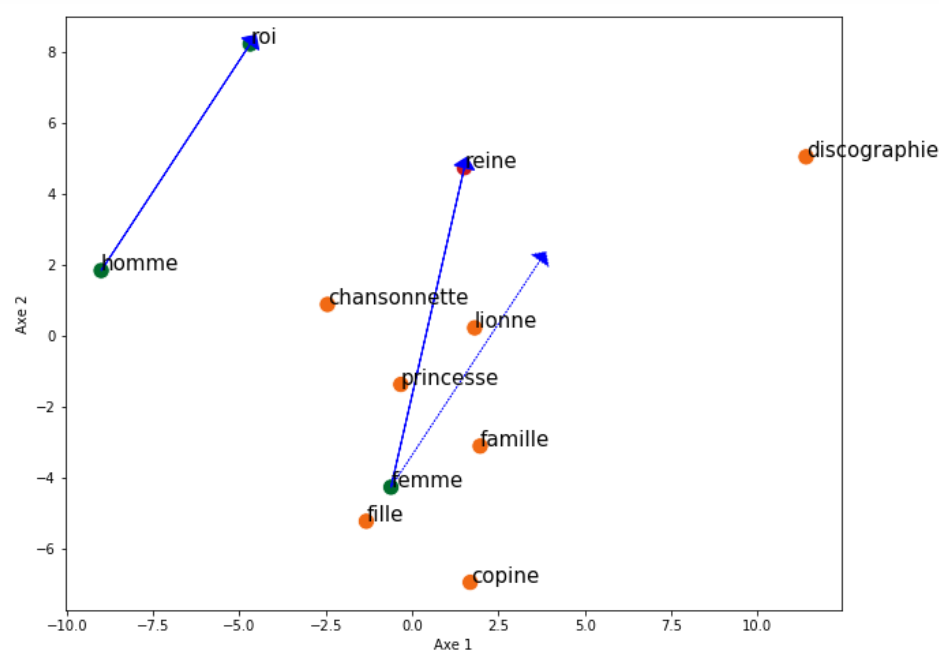
\includegraphics[width=0.92\linewidth]{img/acp_reine.png}
  \captionof{figure}{\ $\protect\overrightarrow{Roi} - \protect\overrightarrow{Homme} + \protect\overrightarrow{Femme} = $ ?}
  \label{fig:acp_reine}
\end{minipage}%
\begin{minipage}{.5\textwidth}
  \centering
  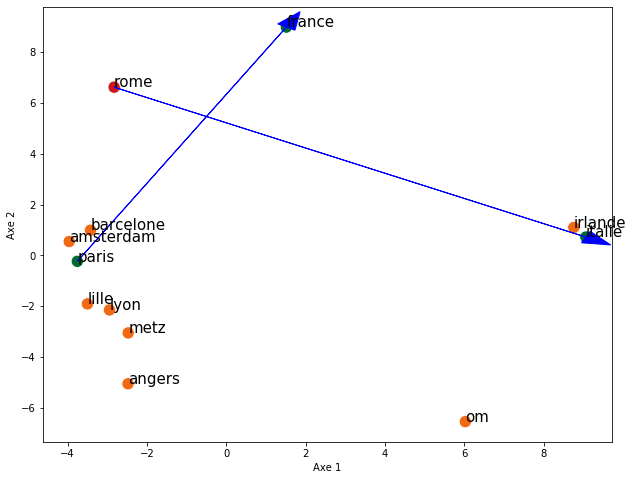
\includegraphics[width=0.85\linewidth]{img/acp_rome.png}
  \captionof{figure}{\ $\protect\overrightarrow{Paris} - \protect\overrightarrow{France} + \protect\overrightarrow{Italie} = $ ?}
  \label{fig:acp_rome}
\end{minipage}
\footnotesize
\emph{Note : Paramètres utilisés : ep = 100 / w = 4 / lr = 0,02 / dim = 100.\newline
Les mots en vert correspondent à ceux présents dans l'opération, le mot en rouge le mot que l'on serait supposé trouver et les mots en orange les 10 mots les plus proches du résultat de l'opération vectorielle.}
\end{figure}

\section{Analyse des sentiments}\label{sec:sentimentalAnalysis}

\subsection{\texorpdfstring{Prédire le sentiment d'un tweet à partir des
\emph{word-embeddings}}{Prédire le sentiment d'un tweet à partir des word-embeddings}}\label{pruxe9dire-le-sentiment-dun-tweet-uxe0-partir-des-word-embeddings}

Nous cherchons dans cette partie à prédire le sentiment associé à un
tweet. Nous nous intéresserons ici à 2 sentiments possibles : +1 quand
le tweet est jugé positif, -1 quand il est jugé négatif. D'une manière
générale, on se demande comment, à partir des mots d'un tweet, on peut
prédire son sentiment. À partir de la base de tweets de la SNCF, nous
allons donc chercher à construire le meilleur modèle de prédiction de
sentiments. Nous comparerons alors deux approches : un première basée
sur les sentiments moyens de chaque mot des tweets et l'autre basée sur
les \emph{word-embeddings}.

\subsubsection{Prédiction à partir du sentiment moyen des
mots}\label{pruxe9diction-uxe0-partir-du-sentiment-moyen-des-mots}

Un premier modèle de prédiction du sentiment peut être imaginé en
utilisant l'information des tweets labelisés pour déterminer un
sentiment moyen par mot. En effet, dans un premier temps, on peut
regarder pour chaque mot du vocabulaire du corpus le nombre de tweets
positifs (\(nb_+\)) et négatifs (\(nb_-\)) dans lesquels il apparaît et
lui associer un sentiment moyen \(\frac{nb_+ - nb_-}{nb_+ + nb_-}\),
compris entre -1 et 1. Dans un second temps, on peut alors calculer la
moyenne des sentiments des mots d'un tweet, et décider du label du tweet
en fonction : si la moyenne est positive, le tweet sera jugé positif,
sinon, il sera négatif. Autrement dit, considérons un tweet \(t\)
composé des mots \(\{ mot_1 , \dots , mot_n \}\) alors
\(S(t) = 2 \times 1\{ \frac{1}{n} \sum \limits_{i=1}^n \alpha_i \geq 0\} - 1\)
est la prédiction du sentiment du tweet, où \(\alpha_i\) est le
sentiment moyen du \(mot_i\).

Afin d'étudier l'ajustement du modèle, nous séparons le corpus en une
base de \emph{train} composée de 16 004 tweets et une base de
\emph{test} composée de 6 858 tweets. Nous entraînons le modèle sur la
base de \emph{train}, c'est-à-dire que l'on calcule les sentiments
moyens des mots de cette base, puis nous estimons le modèle sur la base
de \emph{test}, c'est-à-dire que l'on prédit pour chaque tweet de cette
base un sentiment, que l'on compare au vrai sentiment. Il peut exister
des mots présents dans la base de \emph{test} qui ne le sont pas dans la
base de \emph{train}, pour ces mots-là on met donc le sentiment moyen à
0. L'application de cette méthode permet d'obtenir une \emph{accuracy},
c'est-à-dire un taux de tweets dont le sentiment est bien prédit, de
\(70,52\%\).

Ce modèle peut cependant être amélioré. En effet, pour l'instant on
compare la moyenne des sentiments des mots de la phrase à un seuil qui
vaut 0. Toutefois, on pourrait essayer d'optimiser ce seuil :
\(\forall \gamma \in [-1;1]\), on définit
\(S_{\gamma}(t) = 2 \times 1\{ \frac{1}{n} \sum \limits_{i=1}^n \alpha_i \geq \gamma\} - 1\)
que l'on utilise pour effectuer une prédiction du sentiment, puis on
sélectionne le \(\gamma\) qui maximise l'\emph{accuracy} sur la base de
\emph{test}.

\begin{figure}
\begin{center}
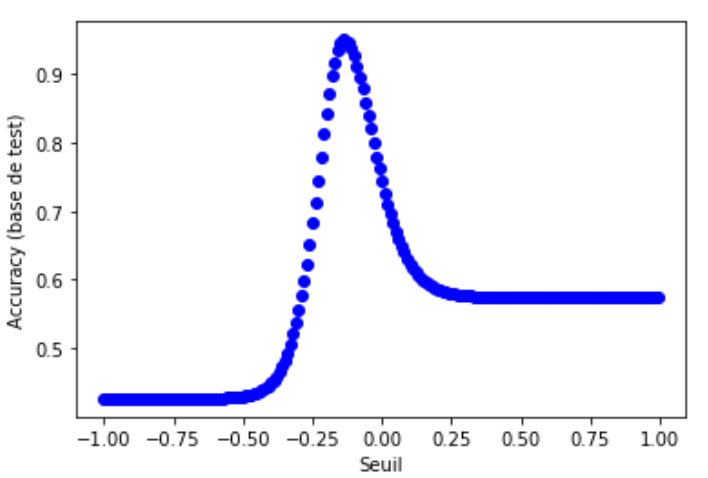
\includegraphics[width=0.5\textwidth]{img/max_baseline.png}
\captionsetup{margin=0cm,format=hang,justification=justified}
\caption{Optimisation du seuil $\gamma$ pour le modèle à partir des sentiments moyens des mots}\label{fig:max_baseline}
\end{center}
\end{figure}

On effectue cette optimisation (figure \ref{fig:max_baseline}) et on
trouve alors que le \(\gamma\) qui maximise l'\emph{accuracy} est
\(\gamma^* = -0.14\), pour une \emph{accuracy} de \(89,08\%\). On
constate donc une nette amélioration par rapport au cas où
\(\gamma = 0\). Nous avons donc ici une premier modèle qui peut servir
de référence pour la suite. Idéalement, nous souhaiterions que le modèle
basé sur les \emph{word-embeddings} soit meilleur que celui-ci.

\subsubsection{\texorpdfstring{Prédiction à partir des
\emph{word-embeddings}}{Prédiction à partir des word-embeddings}}\label{pruxe9diction-uxe0-partir-des-word-embeddings}

Nous nous intéressons maintenant à un modèle basé sur l'utilisation de
nos \emph{word-embeddings}. Afin d'exploiter nos vecteurs, l'idée est
d'utiliser un modèle de régression binaire de estimé sur notre corpus,
en considérant comme prédicteurs chacune des dimensions des vecteurs.
Pour réaliser cette régression, il faut toutefois pouvoir attribuer à
chaque tweet un vecteur et effectuer une forme de \emph{sentence
embedding}. Pour cela, nous décidons d'attribuer à chaque tweet la
moyenne des vecteurs de l'ensemble des mots du tweet. Nous pouvons
ensuite réaliser la régression sur ce vecteur.

Si on note \(Y_i\) le sentiment du tweet \(i\) et
\(X_{i,1}, \dots, X_{i,n}\) chacune des coordonnées du \emph{sentence
embedding} associé au tweet (nous avons ici \(n=100\)), alors on
s'intéresse au modèle
\(Y_i = 1\{ \sum\limits_{i = 1}^n \beta_i X_{i,j} + \epsilon_i \geq 0 \}\)
où \(\epsilon_i\) est le résidu de notre modèle. Nous allons chercher à
estimer, en notant \(F_{\epsilon}\) la fonction de répartition des
résidus :

\begin{equation*}
\mathbb{P}(Y_i = 1 | X_{i,j}) = \mathbb{P}(\sum\limits_{i = 1}^n \beta_i X_{i,j} + \epsilon_i \geq 0 | X_{i,j})
= \mathbb{P}(\sum\limits_{i = 1}^n \beta_i X_{i,j}\geq - \epsilon_i  | X_{i,j}) = F_{\epsilon}(\sum\limits_{i = 1}^n \beta_i X_{i,j})
\end{equation*}

Deux modèles binaires peuvent être utilisés, selon la choix de
\(F_{\epsilon}\) :

\begin{enumerate}
\def\labelenumi{\arabic{enumi}.}
\item
  Le modèle logit : \(F_{\epsilon}(x) = \frac{1}{1 + e^{-x}}\).
\item
  Le modèle probit : \(F_{\epsilon}\) est la fonction de répartition
  d'une loi gaussienne centrée et réduite.
\end{enumerate}

Nous avons donc deux choix de spécification à estimer sur notre corpus,
afin de déterminer la meilleure. En réalité, nous pouvons également nous
interroger sur d'autres paramètres à intégrer au modèle :

\begin{enumerate}
\def\labelenumi{\arabic{enumi}.}
\item
  Les \emph{stop words} : également appelé \og mots vides \fg, ce sont
  des mots communs dont l'analyse est en général inutile car leur
  présence n'apporte pas d'information. Dans notre cas, on peut donc
  penser à estimer le modèle en enlevant du corpus ces
  \emph{stop-words}.
\item
  Les mots inconnus : la base qui a servi à entraîner le modèle des
  \emph{word-embeddings} est différente de celle que l'on utilise pour
  la prédiction des sentiments. Ainsi, il y a des mots de ce corpus pour
  lesquels on ne connaît pas la représentation vectorielle. On peut
  alors décider que la représentation vectorielle des mots inconnus est
  le vecteur nul. Cependant, lorsqu'on a entraîné le modèle
  \emph{Word2Vec} un pré-processing a permis de regrouper les mots très
  peu fréquents au sein d'un même mot clé et le modèle a alors calculé
  une représentation vectorielle commune à tous ces mots. On peut donc
  décider d'attribuer ce vecteur aux mots inconnus, en estimant que
  s'ils sont absents du corpus d'entraînement du modèle \emph{Word2Vec},
  ce sont bien des mots très peu fréquents.
\end{enumerate}

Afin de mener une analyse la plus complète possible, nous avons décidé
d'estimer tous les modèles possibles selon que l'on choisisse :

\begin{enumerate}
\def\labelenumi{\arabic{enumi}.}
\item
  D'inclure ou non les \emph{stop-words} ;
\item
  Le vecteur nul ou le vecteur des mots très peu fréquents estimé pour
  les mots inconnus ;
\item
  Le modèle probit ou logit.
\end{enumerate}

Nous obtenons ainsi 8 modèles à estimer. Pour comparer ces modèles entre
eux, nous avons décidé d'utiliser l'AUC, \emph{Area Under the Curve},
c'est-à-dire l'aire sous la courbe ROC, \emph{receiver operating
characteristic}. \footnote{La courbe ROC permet de représenter pour
  l'ensemble des seuils possibles l'évolution du nombre de vrais
  positifs en fonction du nombre de faux positifs. L'AUC, l'aire sous
  cette courbe, est donc compris entre 0 et 1 (le modèle qui prédirait
  de façon aléatoire 1 ou -1 a un AUC de 0,5).} Nous effectuons alors
une validation croisée, pour chacun de nos 8 modèles, en se basant sur
l'AUC. Nous nous intéressons également à des critères économétriques
afin de déterminer la meilleure représentation entre le modèle logit et
le modèle probit.

Nous obtenons alors les résultats suivants :

\begin{enumerate}
\def\labelenumi{\arabic{enumi}.}
\item
  Il ne semble pas utile d'enlever les \emph{stop words} pour améliorer
  les résultats. Ceci peut s'expliquer car certains \emph{stop-words}
  peuvent peut-être renseigner sur un sentiment. Ainsi, le mot \og pas
  \fg est un \emph{stop-word} mais renseigne plutôt sur des tweets
  négatifs (son sentiment moyen dans le corpus est de -0.25). De même,
  on peut penser que les phrases contenant du futur ou du conditionnel
  renvoie à des sentiments différents.
\item
  Il apparaît meilleur d'affecter aux mots inconnus le vecteur des mots
  peu fréquents estimé par le modèle \emph{Word2Vec} que de leur
  attribuer le vecteur nul. On aurait pu intuitivement penser qu'en
  l'absence d'information sur un mot, il est préférable de lui attribuer
  un vecteur nul afin qu'il n'influe pas sur la décision du sentiment.
  Cependant, cela ne se vérifie pas empiriquement. Cela veut peut-être
  signifier que le vecteur associé aux mots très peu fréquents estimé
  par notre modèle \emph{Word2Vec} capture bien la rareté du mot et que
  les mots peu fréquents ont peut-être tendance à être plus positifs ou
  plus négatifs et non neutres.
\item
  Utiliser un modèle logit permet d'obtenir de meilleurs résultats qu'en
  utilisant un modèle probit. En effet, à la fois les AUC et les
  critères économétriques sont meilleurs pour les modèles logit, quels
  que soient les choix faits par ailleurs sur les \emph{stop words} et
  les mots inconnus.
\end{enumerate}

Finalement, nous utiliserons donc par la suite le modèle estimé par une
\textbf{régression logit} sur la base en \textbf{gardant les
\emph{stop-words} } et en affectant aux mots inconnus dans le modèle
\emph{Word2Vec} le \textbf{vecteur des mots très peu fréquents} estimé
par ce dernier.

L'application de ce modèle à la même base \emph{test} que le modèle basé
sur les sentiments moyens des mots donne une \emph{accuracy} de
\(68,71\%\). Nous obtenons de moins bons résultats en utilisant le
modèle basé sur les \emph{word-embeddings}. Nous allons maintenant
essayer d'analyser ces résultats.

\subsubsection{\texorpdfstring{Une cause des mauvaises prédictions : le
\emph{domain
shift}}{Une cause des mauvaises prédictions : le domain shift}}\label{une-cause-des-mauvaises-pruxe9dictions-le-domain-shift}

Les techniques d'apprentissage automatique sont souvent confrontées à un
défi majeur : le fait que les modèles soient entraînés sur des données
différentes de celles que l'on va effectivement utiliser : c'est ce que
l'on appelle le « \emph{dataset shift} »\footnote{Les éléments en lien
  avec le \emph{dataset shift} proviennent de \cite{Candela}}. Bien que
des solutions comme la correction de biais de sélection des
échantillons, ou encore celle des données déséquilibrées, soient
étudiées depuis de nombreuses décennies dans le monde de la statistique,
certains autres problèmes, comme celui du changement de domaine
(\emph{domain shift}) émergent depuis plus récemment suite à
l'utilisation croissante des méthodes de \emph{machine learning}.

Le changement de domaine se caractérise par un changement de la nature,
du « domaine » des données utilisées. Dans le cas de
\emph{deep-learning} sur des données de photographie, il pourrait par
exemple s'agir de traiter de corpus de photos prises par des appareil
photo calibrés de manière différentes (contraste, luminosité\ldots{}) .
Dans notre cas précis, il s'agit de la différence entre les données de
tweets publiés en France entre 2013 et 2017 et les données de tweets de
la SNCF, qui portent sur un sujet très spécifique et pour lesquels
certains mots ont peut-être une interprétation spécifique en termes de
sentiments. Modéliser le « domain shift » implique donc d'estimer le
passage d'une représentation à une autre en utilisant des informations
de distribution. \footnote{La correction gamma (représentation
  paramétrique non linéaire de l'intensité des pixels) est par exemple
  une manière de pouvoir traiter le « domain shift » lié à l'utilisation
  d'appareil photos différents.} Dans ce qui suit, l'idée n'est pas de
modéliser mathématiquement\footnote{Pour modéliser mathématiquement de
  manière relativement « grossière » un \emph{domain shift}, il
  s'agirait de considérer par exemple une variable latente « idéale »
  \(x_0\) (une base de tweets de référence), jamais observée mais qui
  influerait sur \(y\) (l'indice mensuel). Nous observons uniquement
  \(x\) telle \(x=F(x_0)\) avec \(F\) qui représente la transformation
  de la base de tweets de référence à la base de tweets réellement
  utilisée, qui peut varier en fonction de la base de données \(x\)
  utilisée. La distribution \(P(y|x_0)\) (de l'indice mensuel sachant le
  jeu de tweets idéal utilisé) est considérée comme étant la même pour
  les deux jeux de tweets utilisée (base « sncf » et base de tweets
  postés en France entre 2013 et 2017). En revanche, cette distribution
  est modifiée si F est modifiée.} le \emph{domain shift} des deux bases
de tweets mais de présenter quelques statistiques descriptives
illustrant ce phénomène.

Pour ce faire, \ldots{}

\subsection{Sentiments des tweets et enquête de conjoncture auprès des
ménages
{[}Alain{]}}\label{sentiments-des-tweets-et-enquuxeate-de-conjoncture-aupruxe8s-des-muxe9nages-alain}

\section*{Conclusion {[}sûrement
Kim{]}}\label{conclusion-suxfbrement-kim}
\addcontentsline{toc}{section}{Conclusion {[}sûrement Kim{]}}

\newpage

\appendix


\section{Comment évaluer le modèle ?}\label{annexe:commentEvaluer}

\subsection{Distance entre deux mots}\label{distance-entre-deux-mots}

L'un des enjeux principaux du modèle étant de pouvoir estimer la
proximité entre deux vecteurs-mots, nous pouvons tout d'abord mesurer
cette dernière par des calculs de distance.

Il existe différents types de distances. Chacune d'elles possède des
propriétés intéressantes et s'adaptent plus ou moins bien au problème
traité. Nous avons ici retenu deux distances classiquement utilisées :

\begin{itemize}
\tightlist
\item
  \textbf{la distance euclidienne} :
  \(d_{e}(\vec{u},\vec{v}) = \left\| \vec{u} - \vec{v} \right\|_2\)\\
  Un problème est que la longueur du vecteur mot, captée dans le cas de
  la distance euclidienne, est positivement corrélée à la fréquence
  d'apparition du mot (\cite{Schakel}). Cette information peut s'avérer
  utile dans l'analyse de la signification des mots, notamment lorsque
  l'on effectue des opérations sur les vecteurs (comme l'exemple de
  \(\overrightarrow{Paris} - \overrightarrow{France} + \overrightarrow{Italie} = \overrightarrow{Rome}\)
  dans \cite{Mikolov}).\\
  Toutefois, cette dépendance à la fréquence d'apparition peut également
  fausser l'analyse. C'est pourquoi nous avons choisi, par la suite, de
  normaliser les vecteurs :
  \[ d_{e}(\vec{u},\vec{v}) = \left\| \frac{\vec{u}}{\left\| \vec{u} \right\|_2} - \frac{\vec{v}}{\left\| \vec{v} \right\|_2}  \right\|_2\]
\item
  \textbf{la similarité cosinus} :
  \(d_{c}(\vec{u}, \vec{v}) = \frac{\vec{u}.\vec{v}}{\left\| \vec{u} \right\|_2 \left\| \vec{v} \right\|_2 }\).\\
  La similarité cosinus correspond au produit scalaire entre les deux
  vecteurs normalisés. Elle mesure ainsi l'angle formé entre deux
  vecteurs-mots.\\
  C'est la distance que de nombreux papiers fondateurs de la méthode
  \emph{Word2Vec} (comme \cite{Mikolov} ou \cite{Levy}) utilisent, avec
  l'argument selon lequel les mots apparaissant dans des contextes
  similaires sont groupés dans la même direction durant l'entraînement.
  Une similarité est proche de \(+1\) si deux mots sont positivement
  reliés (proches), de \(-1\) s'ils sont négativement reliés (éloignés)
  et de 0 s'ils ne sont pas \og reliés \fg{}.\\
  Il est toutefois délicat d'interpréter une similarité proche de
  \(-1\). On pourrait intuitivement penser à des antonymes, comme
  \og grand \fg{} et \og petit \fg{}, mais en pratique, les antonymes
  sont susceptibles d'apparaître dans des contextes semblables et sont
  donc bien souvent positivement corrélés.
\end{itemize}

\subsection{Analyse en Composantes
Principales}\label{analyse-en-composantes-principales}

Une fois le modèle \emph{Word2Vec} entraîné, nous obtenons des
\emph{word-embeddings} pour chacun de nos mots, représentés par des
vecteurs de grandes dimensions (20, 50 ou même supérieures à 100).

Dès lors, il devient complexe de bien observer la proximité entre deux
mots. C'est pourquoi il devient utile de mobiliser des méthodes de
réduction de dimensions comme l'analyse en composantes principales
(ACP). En effet, l'objectif premier de cette méthode est de projeter un
nuage de points sur un espace de dimension inférieure. Cela permet de
rendre l'information moins redondante et plus visuelle, tout en étant le
plus proche possible de la réalité.

Considérons le cas où nous disposons de \(n\) individus (dans notre cas
les mots) et de \(p\) variables (dans notre cas, leurs composantes ou
dimensions issues du modèle \emph{Word2Vec}). On note \(X = (x_{ij})\)
la matrice de taille \((n,p)\) des données brutes, où \(x_{ij}\)
représente la valeur de la \(j\)-ème variable pour le \(i\)-ème
individu. Mathématiquement, pour définir l'ACP, on définit deux espaces
:

\begin{itemize}
\item
  L'\emph{espace des individus}, de dimension \(p\), auquel on associe
  la métrique \(M\) utilisée pour le produit scalaire. Dans la suite
  nous utiliserons \(M =I_p\) la matrice identité. La norme et le
  produit scalaire associés à \(M\) sont donc euclidiens.
\item
  L'\emph{espace des variables}, de dimension \(n\), auquel associe la
  métrique \(N=diag(p_1,...,p_n)\) avec \(\sum_{i=1}^np_i=1\). La
  matrice \(N\) représente le poids donné à chaque individu. Par
  simplification nous utiliserons ici des poids uniformes :
  \(N=\frac{1}{n}I_n\). Afin de donner le même poids à toutes les
  variables, chaque variable est centrée-réduite : cela revient à
  centrer-réduire les colonnes de notre matrice \(X\). Nous notons
  \(Z =\bar X= (z_{ij})\) la matrice des données centrées et
  réduites\footnote{Nous travaillons ici dans le cadre d'une ACP normée
    où la matrice \(X\) a été centrée puis réduite. La réduction de
    \(X\) a modifié les distances initiales entre individus
    (\(\langle z_i,z_{i'}\rangle_M \neq \langle x_i,x_{i'}\rangle_M\)).
    Cela n'aurait pas été le cas si la matrice \(X\) avait été
    uniquement centrée (ACP non normée).}.
\end{itemize}

Pour toute métrique \(D\) (\(D=N\) ou \(D=M\)), on associe le produit
scalaire \(\langle x,y\rangle_{D} = {}^t\!xD y\). La construction des
axes de l'ACP est faite par projection orthogonale. La projection
orthogonale d'un individu \(i\) (vecteur ligne) \(z_i\) sur une droite
de vecteur directeur unitaire \(v\) vaut
\(\langle {}^tz_i,v\rangle_{M}=z_i\times v\) et les coordonnées de
projection des \(n\) individus valent \(Zv\).

Les vecteurs directeurs des axes sont définis de manière à maximiser la
dispersion du nuage (son inertie\footnote{}) des individus projetés et
conserver ainsi au mieux les distances entre les individus.
L'inertie\footnote{La dispersion d'un nuage de points unidimensionnel
  par rapport à sa moyenne se mesure par la variance. Dans le cadre
  multidimensionnel, la dispersion du nuage par rapport à son barycentre
  \(\bar z\) se mesure par l'inertie, qui généralise la variance.} se
définit alors comme :

\begin{align*}
I(Z) &= \sum_{i = 1}^n p_i\|z_i-\bar{z}\|_M^2 \text{ avec }
  \bar{z} = 
  \begin{pmatrix}\bar z_{1} \\
    \vdots \\ \bar z_{p}
  \end{pmatrix} =
  \begin{pmatrix}\frac 1 n \sum_{i=1}^n z_{i,1} \\
    \vdots \\ \frac 1 n \sum_{i=1}^n z_{i,p}
  \end{pmatrix} (= 0_{\mathbb R^p}\text{ dans notre cas})
\\&=\sum_{i = 1}^n \frac 1 n \sum_{j=1}^p (z_{i,j} -  \bar{z}_j)^2  \text{ car }M=I_p 
\\&=\sum_{j = 1}^p \frac 1 n \sum_{i=1}^n (z_{i,j} -  \bar{z}_j)^2
\\&=\sum_{j = 1}^p Var(z^j)\text{, avec } z^j = 
  \begin{pmatrix} z_{1,j} \\ \vdots \\  z_{n,j} 
  \end{pmatrix}
\\ &= p \text{ car les variables sont réduites}
\end{align*}

On trouve tout d'abord le vecteur directeur \(v_1\) qui orientera le
premier axe de l'ACP grâce au programme suivant : \[
v_1 =\underset{\| v \|_M = 1}{\mathrm{argmax~}} 
\underbrace{\|Zv\|_N}_{=Var(Zv)} =\underset{\| v \|_M = 1}{\mathrm{argmax~}} ^t\!vR v 
\] où \(R = Var(Z) = \frac{1}{n} ^t\!Z Z\) est la matrice des
corrélations entre les \(p\) variables.

Puis, on choisit \(v_2\) orthogonal à \(v_1\) tel que l'inertie soit
toujours maximisée : \[
v_2 =\underset{ \| v \|_M = 1,\,v \perp v_1}{\mathrm{argmax}}\;  Var(Zv)
\] En procédant de manière séquentielle, on obtient \(q < r\) axes
orthogonaux avec \(r = rg(Z)\) et \(q\) choisi par le
statisticien\footnote{Différentes méthodes existent afin de déterminer
  le \(q\) optimal, comme la règle de Kaiser ou encore celle du coude.}.

On peut montrer que \(\forall k < q\) :

\begin{itemize}
\tightlist
\item
  \(v_k\) est un vecteur propre associé à la k\ieme{} valeur propre
  \(\lambda_k\) de \(R\) (les valeurs propres étant rangées par ordre
  décroissant) ;
\item
  la composante principale \(Zv_k\) est centrée et
  \(V(Zv_k)= \lambda_k\) ;
\item
  les \(Zv_k\) ne sont pas corrélés entre eux.
\end{itemize}

On obtient alors la matrice \(F = ZV\) des nouvelles coordonnées
factorielles des individus, avec \(V = (v_1,\dots,v_q)\) la matrice des
vecteurs propres.

Nous utilisons ici l'ACP en vue d'identifier les individus (ici, nos
mots) qui sont proches. Pour ce faire, il suffit de représenter les
coordonnées factorielles de la matrice \(F\) dans des repères, en
général en 2 dimensions pour une question de lisibilité. Deux mots
apparaissant dans des contextes similaires seront proches sur ce repère
et orientés dans la même direction.

Enfin, pour juger de la qualité de la réduction de dimension, on calcule
souvent la proportion de l'inertie totale expliquée par les \(q\)
premières composantes principales.

\[ \frac{V(F)}{I(Z)} = \frac{\sum \limits_{i = 1}^q \lambda_i}{p}\]

\subsection{\texorpdfstring{Algorithme \emph{t-distributed Stochastic
Neighbor
Embedding}}{Algorithme t-distributed Stochastic Neighbor Embedding}}\label{algorithme-t-distributed-stochastic-neighbor-embedding}

Bien que l'ACP soit une première manière de résumer l'information
contenue dans nos vecteurs, elle présente des limites, notamment dans
les vecteurs aux trop grandes dimensions, pour lesquels l'inertie des
premiers axes de l'ACP peut se révéler faible.

Pour combler ces lacunes, un autre algorithme de réduction de dimension
peut être utilisé, celui dit du \emph{t-distributed Stochastic Neighbor
Embedding} (t-SNE). Contrairement à l'ACP, cet algorithme est
stochastique et non-linéaire et il favorise l'apparition de groupes de
mots proches. Sa philosophie demeure cependant identique : représenter
dans un espace à dimension réduite notre nuage de points de manière à
repérer les mots proches.

La première étape de l'algorithme consiste à calculer les similarités
entre les \(n\) vecteurs-mots \((x_i)_{i=1...n}\). La similarité entre
\(x_i\) et \(x_j\) se mesure comme étant la probabilité conditionnelle
\(p_{j|i}\) de choisir \(x_j\) comme voisin de \(x_i\), si les voisins
étaient tirés au sort selon une loi
\(\mathcal{N}(x_i, \sigma_i)\)\footnote{\(\sigma_i\) doit être calculé
  de manière à adapter la loi conditionnelle aux données. Une faible
  dispersion autour de \(x_i\) entraînera un \(\sigma_i\) faible et
  réciproquement. Il s'agit de trouver le \(\sigma_i\) qui minimise ce
  qui est appelé en théorie de l'information la \og perplexité \fg{},
  c'est-à-dire un indicateur qui décrit à quel point une distribution de
  probabilité réussit à prédire un échantillon.} :

\[ p_{j|i} = \frac{
\exp\left(-\frac{(d_e(x_i - x_j))^2}{2\sigma_i^2}\right)
}{
\sum_{k \neq i}
\exp\left(-\frac{(d_e(x_i - x_k))^2}{2\sigma_i^2}\right)
}\]

La seconde étape de l'algorithme consiste à trouver le nouvel espace de
projection à faible nombre de dimensions. On appellera \(g_i\) les
\(x_i\) projetés dans cet espace que l'on cherche à déterminer. On
calcule maintenant les probabilité conditionnelles \(q_{j|i}\) de
choisir \(g_j\) comme voisin de \(g_i\) en supposant que les \((g_i)_i\)
suivent cette fois-ci une distribution de \emph{Student} -- d'où le nom
de l'algorithme -- plutôt qu'une loi gaussienne\footnote{Dans un espace
  à faible dimension, la dispersion des vecteurs est réduite. La
  distribution de Student possède des queues plus épaisses que la loi
  normale, ce qui permet de mieux différencier les vecteurs distants des
  vecteurs similaires.}.

\[ q_{j|i} = \frac{(1+ (d_e(g_i - g_j))^2)^{-1}}{\sum_{k \neq i}{(1+ (d_e(g_i - g_k))^2)^{-1}}}\]

Afin d'obtenir les \(g_i\), on minimise, par descente de gradient, la
divergence de Kullback--Leibler entre les distributions de probabilité P
et Q des \(p_{ij}\) et \(q_{ij}\) définis par :
\[KL(P,Q) = \sum_{i \neq j} { p_{ij} \log{\frac{p_{ij}}{q_{ij}}}} \qquad\text{avec}\qquad p_{ij} = \frac{p_{i|j} + p_{j|i}}{2n}\]

Comme dans l'algorithme de l'ACP, l'algorithme de t-SNE nous permet
d'obtenir une nouvelle projection des \(x_i\). Il faut cependant
analyser avec précaution ses résultats. L'algorithme n'étant pas
linéaire, l'interprétation de la taille des \emph{clusters} obtenus ou
de la distance qui les sépare n'est alors pas directe.

\subsubsection{Jugement humain}\label{sec:jugementHumain}

Les \emph{word-embeddings} obtenus par \emph{Word2Vec} sont censés
regrouper les mots qui apparaissent dans un contexte similaire. Une
dernière façon de vérifier la qualité de nos vecteurs-mots est de les
comparer à un jugement humain. Pour ce faire, nous utilisons la liste de
référence RG-65 pour le français\footnote{Le RG-65 a fait appel à 18
  évaluateurs humains. La base, initialement mobilisée dans un article
  anglophone (\cite{Rubenstein}) a été traduite de l'anglais.}
(\cite{Boumedyen}). Elle contient 65 paires de noms communs (tableau
\ref{table:human_judgement}) évaluées sur une échelle de 0 (non liés) à
4 (très liés).

Nous calculons ensuite la corrélation de Spearman entre les similarités
cosinus de ces différentes paires issues de notre modèle (notées ici
\((X_i)_{i=1..n}\)) et les scores proposés ci-dessus par des êtres
humains (notés ici \((Y_i)_{i=1..n}\)).

La corrélation de Spearman est égale au coefficient de corrélation de
Pearson calculé sur les variables de rang. \[
r_s = \mathrm{corr}(\mathrm{rg}_X, \mathrm{rg}_Y) = 
\frac{\mathrm{cov}(\mathrm{rg}_X, \mathrm{rg}_Y)}{
\sigma_{\mathrm{rg}_X} \sigma_{\mathrm{rg}_Y}
}
\] La variable de rang \(\mathrm{rg}_{X_i}\) est définie telle que
\(\mathrm{rg}_{X_i}=j \iff X_i = X_{(j)}\) (\(X_i\) est la \(j\)ème plus
petite variable).

Pour tester la significativité de ce coefficient, nous utilisons la loi
sous \((H_0)\) de la statistique de test
\(z = \arctanh(r_s) = \frac{1}{2} \ln\frac{1+r}{1-r} \overset{H_0}{\sim}\mathcal{N}(0, \frac{1}{n-3})\)
et obtenons l'intervalle de confiance suivant :

\[
IC_\alpha (r_s) = \left[\tanh\left(z-\frac{q_{1-\frac{\alpha}{2}}}{\sqrt{n-3}}\right),
\tanh\left(z+\frac{q_{1-\frac{\alpha}{2}}}{\sqrt{n-3}}\right)\right]
\] avec \(q_{1-\frac{\alpha}{2}}\) le quantile d'ordre
\(1-\frac{\alpha}{2}\) d'une loi \(\mathcal{N}(0, 1)\).

\begin{table}
\begin{center}
\begin{tabular}{|c|c|c|}
    \hline
    mot 1 & mot 2 & similarité  \tabularnewline
    \hline
    corde & sourire & 0,00   \tabularnewline
    midi & ficelle & 0,00   \tabularnewline
    \dots & \dots & \dots   \tabularnewline
    corde & ficelle & 3,33   \tabularnewline
    \dots & \dots & \dots   \tabularnewline
    automobile & auto & 3,94   \tabularnewline
    coq & coq & 4,00   \tabularnewline
    \hline
 \end{tabular}
\captionsetup{margin=0cm,format=hang,justification=justified}
\caption{Base de données de jugement humain}\label{table:human_judgement}
\end{center}
\end{table}

\newpage

\nocite{*}

\begin{thebibliography}{999}
\bibitem[Bengio \emph{et al} (2003)]{Bengio} Bengio, Y., Ducharme, R., Vincent, P., Janvin, C. (2003). A Neural Probabilistic Language Model. JMLR, 3:1137–1155. \url{https://papers.nips.cc/paper/1839-a-neural-probabilistic-language-model.pdf}.
\bibitem[Boumedyen Billami \& Gala (2017)]{Boumedyen} Boumedyen Billami, M.,  Gala, N (2017). Création et validation de signatures sémantiques : application à la mesure de similarité sémantique et à la substitution lexicale. TALN 2017. \url{https://hal.archives-ouvertes.fr/hal-01528117/document}.
\bibitem[Candela et al. (2009)]{Candela} Candela, J. Q., Sugiyama, M., Schwaighofer, A., \& Lawrence, N. D. (2009) Dataset shift in machine learning. The MIT Press, 1, 5. \url{http://www.acad.bg/ebook/ml/The.MIT.Press.Dataset.Shift.in.Machine.Learning.Feb.2009.eBook-DDU.pdf}.
\bibitem[Hutter, Hoos \& Leyton-Brown (2014)]{Hutter} Hutter, F., Hoos, H., Leyton-Brown, K., (2014). An Efficient Approach for Assessing Hyperparameter Importance. PMLR 32(1):754-762. \url{http://proceedings.mlr.press/v32/hutter14.pdf}.
\bibitem[Jurafsky \& Martin (2019)]{Jurafsky} Jurafsky, D., Martin, J. H. (2019). Speech and Language Processing (3rd ed. draft). Prentice Hall. \url{https://web.stanford.edu/~jurafsky/slp3/edbook_oct162019.pdf}.
\bibitem[Levy \& Golberg (2015)]{Levy} Levy, O., Golberg, Y. (2015). Neural Word Embedding as Implicit Matrix Factorization.
\url{https://papers.nips.cc/paper/5477-neural-word-embedding-as-implicit-matrix-factorization.pdf}.
\bibitem[Levy \& Golberg (2014)]{Levy2} Levy, O., Golberg, Y. (2014). Dependency-based word embeddings. ACL. \url{http://papers.nips.cc/paper/5477-neural-word-embedding-as-implicit-matrix-factorization.pdf}.
\bibitem[Mikolov \emph{et al} (2013a)]{Mikolov} Mikolov, T.,  Chen, K., Corrado, G., Dean, J. (2013a). Efficient Estimation of Word Representations in Vector Space. arXiv:1301.3781. \url{https://arxiv.org/pdf/1301.3781.pdf}.
\bibitem[Mikolov \emph{et al} (2013b)]{MikolovNS} Mikolov, T., Sutskever, I., Chen, K., Corrado, G. S., and Dean, J. (2013b). Distributed representations of words and phrases and their compositionality, arXiv:1310.4546. \url{https://arxiv.org/pdf/1310.4546.pdf}.
\bibitem[Pennington, Socher \& Manning (2014)]{Pennington} Pennington, J., Socher, R., Manning, C. D., (2014).  Glove: global vectors for word representation. Proc. of EMNLP,1532 – 1543. \url{https://www.aclweb.org/anthology/D14-1162.pdf}.
\bibitem[{\v R}eh{\r u}{\v r}ek \& Sojka (2010)]{Rehurek} {\v R}eh{\r u}{\v r}ek, R.,  Sojka, P. (2010). Software Framework for Topic Modelling with Large Corpora. Proceedings of LREC 2010 workshop New Challenges for NLP Frameworks. p. 46--50, 5 pp. ISBN 2-9517408-6-7. \url{https://is.muni.cz/publication/884893/en}.
\bibitem[Rubenstein \& Goodenough (1965)]{Rubenstein} Rubenstein, H.,  Goodenough, J. B. (1965). Contextual Correlates of Synonymy. Commun. ACM, 8 (10), 627–633. \url{https://dl.acm.org/doi/10.1145/365628.365657}.
\bibitem[Schakel \& Wilson (2015)]{Schakel} Schakel, A. M., Wilson, B. J. (2015). Measuring Word Significance using Distributed Representations of Words. arXiv:1508.02297. \url{https://arxiv.org/pdf/1508.02297v1.pdf}.
\end{thebibliography}

\end{document}
